\documentclass[
  digital, %% The `digital` option enables the default options for the
           %% digital version of a document. Replace with `printed`
           %% to enable the default options for the printed version
           %% of a document.
  color,   %% Uncomment these lines (by removing the %% at the
           %% beginning) to use color in the digital version of your
           %% document
  table,   %% The `table` option causes the coloring of tables.
           %% Replace with `notable` to restore plain LaTeX tables.
  %twoside, %% The `twoside` option enables double-sided typesetting.
           %% Use at least 120 g/m² paper to prevent show-through.
           %% Replace with `oneside` to use one-sided typesetting;
           %% use only if you don’t have access to a double-sided
           %% printer, or if one-sided typesetting is a formal
           %% requirement at your faculty.
  oneside, % temp for digital version
  lof,     %% The `lof` option prints the List of Figures. Replace
           %% with `nolof` to hide the List of Figures.
  lot,     %% The `lot` option prints the List of Tables. Replace
           %% with `nolot` to hide the List of Tables.
  %% More options are listed in the user guide at
  %% <http://mirrors.ctan.org/macros/latex/contrib/fithesis/guide/mu/fi.pdf>.
]{fithesis3}
%% The following section sets up the locales used in the thesis.
\usepackage[resetfonts]{cmap} %% We need to load the T2A font encoding
\usepackage[T1,T2A]{fontenc}  %% to use the Cyrillic fonts with Russian texts.
\usepackage[
  main=english, %% By using `czech` or `slovak` as the main locale
                %% instead of `english`, you can typeset the thesis
                %% in either Czech or Slovak, respectively.
  czech         %% The additional keys allow
]{babel}        %% foreign texts to be typeset as follows:
%%
%%   \begin{otherlanguage}{czech}   ... \end{otherlanguage}
%%
%% The following section sets up the metadata of the thesis.
\thesissetup{
    date        = \the\year/\the\month/\the\day,
    university  = mu,
    faculty     = fi,
    type        = bc,
    author      = Jan Rychlý,
    gender      = m,
    advisor     = {doc. Mgr. Jan Obdržálek, PhD.},
    title       = {Game development in Haskell},
    % TeXtitle    = {Game development in Haskell},
    keywords    = {Haskell, functional paradigm, game development,
                   Entity-Component-System, apecs, parallelism, monadic abstraction},
    TeXkeywords = {Haskell, functional paradigm, game development,
                   Entity\textendash{}Component\textendash{}System,
                   apecs, parallelism, monadic abstraction},
    abstract    = {%
        Purely functional programming offers many benefits,
        like briefer, safer, and more understandable code.
        This thesis aims to show that these benefits also
        apply to developing smaller-scale video games in Haskell and,
        more importantly, that the drawbacks do not outweigh them.

        We present two implementations of a simple game.
        The first one uses Entity\textendash{}Component\textendash{}System
        provided by the apecs library,
        and the second focuses on pure-style, parallelism-capable design.
        Furthermore, we compare the two together with
        an already existing imperative implementation.
        We show that Haskell's powerful type system,
        including its typeclasses and monadic abstraction,
        is of especially great value for a good design
        of real-time interactive applications such as games.
        At last, we discuss how our findings may scale up.
    },
    thanks      = {%
      I want to thank my advisor, doc. Mgr. Jan Obdržálek, PhD., for his invaluable feedback,
      patience, and encouragement. I also want to thank my colleagues at KISK
      for tolerating my lousy tempo as I was finishing this thesis.
      Finally, special thanks go to my fiancée for putting up with
      the lengthy explanations of my excitement over programming and
      my friends and family for all their support
      --- especially my parents for not letting me starve
      to death while working on this thesis.
    },
    bib         = bibliography.bib,
    %% Uncomment the following line (by removing the %% at the
    %% beginning) and replace `assignment.pdf` with the filename
    %% of your scanned thesis assignment.
%%    assignment         = assignment.pdf,
}
\usepackage{makeidx}      %% The `makeidx` package contains
\makeindex                %% helper commands for index typesetting.
%% These additional packages are used within the document:
\usepackage{paralist} %% Compact list environments
\usepackage{amsmath}  %% Mathematics
\usepackage{amsthm}
\usepackage{amsfonts}
\usepackage{url}      %% Hyperlinks
\usepackage{markdown} %% Lightweight markup
\usepackage{tabularx} %% Tables
\usepackage{tabu}
\usepackage{booktabs}

\usepackage[newfloat, chapter]{minted} %% source code highlighting
\usemintedstyle{vs}
\usepackage{xcolor}
\usepackage{hyperref}
\usepackage{dirtytalk}
\usepackage{dirtree} %% fancy directory structure

\usepackage{floatrow} %% Putting captions above tables
\floatsetup[table]{capposition=top}



% C++ macros
\newcommand{\cpp}{C\nolinebreak\texttt{+}\nolinebreak\texttt{+}}
\newminted[cppblock]{cpp}{breaklines}
\newmintinline[inlinecpp]{cpp}{breaklines}

% Haskell macros
\definecolor{haskellbg}{rgb}{0.95,0.95,0.96}
\newminted[haskell]{haskell}{
    % frame = leftline,
    % bgcolor = haskellbg,
    breaklines,
    % breakanywhere,
    % escapeinside=//,
}
\newmintinline[inlinehs]{haskell}{breaklines}
\newcommand{\packagename}{\mintinline{Haskell}}

\newminted[term]{console}{breaklines}

\newcommand{\vs}{vs.\ }




\begin{document}


% ====================================
% Introduction
% ====================================
\chapter*{Introduction}
\addcontentsline{toc}{chapter}{Introduction}
\label{chptr:introduction}

% // introduction draft written for the VB000 assignment

Video games are a special kind of application that many consider an art form
and rewarding to develop. However, they generally involve a complex system
with a non-trivial state, a certain amount of pseudo-randomness,
and user/player input handling. This makes for non-deterministic
programs that are usually incredibly difficult to test efficiently.

Conversely, functional programming strives to eliminate
mutable state and make code more deterministic, which allows for
programs to be safer and easier to test.
These and other benefits have naturally led to people
trying out game development in functional languages, but
it remains mostly a matter of passion projects.
That said, even though the vast majority of the video game industry
still uses imperative languages like \cpp{}, the communities
\emph{are} very active, and there are hundreds of games,
blog posts, and libraries that help with
game programming in functional languages.

The focus of this thesis narrows down to exploring game development
in Haskell in the context of small-scale 2D games. The goal is
to give an overview of the process, then compare this approach
to a more conventional and imperative one
and ultimately highlight the features of Haskell that are beneficial
and those that become hurdles in the context of programming a video game.

This is done through reimplementing a single game with an already existing
imperative implementation in Haskell,
first using the apecs\footfullcite{apecsrepo} library
and for a second time without it. After a further discussion
about chosen technologies in the following chapter,
said three implementations are described and analyzed
in chapters \ref{chptr:hasteroids}, \ref{chptr:purity}, and~\ref{chptr:impasteroids}.
Then they are more closely compared
and the pros and cons of Haskell in game development are
evaluated and demonstrated in Chapter~\ref{chptr:evaluation}.

We find that the apecs library makes developing games
in Haskell much more approachable, and provides good performance.
On the other hand it leads the programmer against the functional philosophy, and using it
will generally result in very imperative code wrapped in monads
that lacks the expressiveness and apparent safeness of regular Haskell.
Yet, from the second implementation, we learn that
some use of monads is beneficial, and it makes the code cleaner, more elegant,
and more flexible. It could also be modified to use parallelism for
world updating and detecting collisions since the functions are all pure and compartmentalized.
Furthermore, we discuss what a middle-ground solution may look like
with the use of typeclasses and monads, and how our findings may scale to larger games.
In both cases, the development was
mostly a smooth experience without a single major hiccup,
unlike what often happens when dealing with a \cpp{} compiler.




% ====================================
% CHAPTER 1 - Deeper introduction
% ====================================
\chapter{Motivation and used methods}
\label{chap:motivationandmethods}


\section{Why functional programming matters}
\label{sect:whyfpmatters}

Functional languages are a subset of declarative languages, where the
programmer states \say{what} instead of \say{how}. Unlike in imperative languages,
we \emph{declare} what we want a program to return by combining functions (other declarations)
instead of giving the computer serialized instructions (\emph{imperatives}).
That is manifested in the lack of assignment statements and lesser control structures.
Once variables are assigned their value, it cannot be changed,
and the \say{burden} of prescribing the flow of control
is removed \cite{whyfpmatters}. Moreover, a pure function has no side effects,
and its return value depends solely on its arguments. This makes for deterministic
programs that are easier to test, debug and argue about their correctness.

John Hughes describes the key benefits of the functional paradigm in his paper
\textit{Why Functional Programming Matters} \cite{whyfpmatters}. He first
explains how modularity of code is essential, since
separate modules are easier to write and test and then proceeds
to show how functional programming increases modularity
through higher-order functions and lazy evaluation, demonstrating
their importance on several examples.

Additionally, Haskell is a purely functional programming language that
is also \emph{strongly typed}. This means that one
does not need to worry about memory errors causing crashes because
the type-checker catches everything during compilation.
The types also serve as documentation and can help greatly
with writing and understanding code. At the same time,
the compiler can also infer types, so it
is not necessary to explicitly declare them everywhere.
Furthermore, the type system allows extensive user-defined data types,
which makes the code even more expressive.
All of this potentially increases productivity of a functional programmer even further.


\subsection{Game development specifics}
Functional languages are great tools, but we know that not every tool is
fit for every task. One of the consequences of functional purity is
that the program's state has to be modeled explicitly as an argument
and is therefore immutable. There are monads that help us abstract
from this, but the monads themselves are, in a way, still an explicit workaround.

Conversely, games are real-time, interactive applications often simulating
complex systems and holding a non-trivial state updated many times a second.
Such s state generally involves representing
the game world with all the objects existing in it, their properties and flags,
the current state of the input devices and many other variables. Since its beginning,
the video game industry has been dominated by imperative languages
that make it easy to model a game world and alter it globally through
references and side effects inside decomposed functions. Moreover, because
of their established position, there are many libraries and game engines
with supporting documentation and tutorials. Besides, a company will most likely
have no problem finding skilled \cpp{} programmers with an interest
in the game industry, whereas finding their functional counterparts
might be much more challenging. Additionally, in the case of \cpp{} the performance
also fits the requirements of big games.

However, it does come with a price --- modules of such programs may be
more dependent and entangled, which makes the whole less flexible and with
implicit state more prone to bugs and harder to test and debug.
That is, while testing is already a significant issue due to the nature of video games.
Automated testing is not sufficient, and companies have to hire teams
of game testers to test games manually. And in terms of high performance,
which is generally connected to lower-level languages, developers must
wrestle with the lower-level nature, producing problems as well.
Haskell also has the edge in the area of parallelism and concurrency,
which is becoming more relevant as new hardware keeps increasing in core counts,
and complex, intertwined, imperative systems are challenging to run in parallel.

We can see that video games, like any other software, could benefit from
purely functional design, provided that we are able to model the
game state efficiently enough. Another consideration in the real world
is the available frameworks and whether the cost of potential
pioneering is worth it.


\subsection{Existing work}
\label{sect:existing}
Indeed, people have tried developing games in Haskell, and a decent
progress has been made over the years. There are libraries and engines like Yampa \cite{yamparepo}
and Helm \cite{helmrepo} for functionally reactive programming (FRP) of video games and
other general FRP libraries that have been used to make games, like Elerea \cite{elerearepo}
or Netwire \cite{netwirerepo}. From non-FRP libraries, there is
FunGEn \cite{fungenrepo}, the self-proclaimed oldest Haskell game engine,
apecs \cite{apecsrepo}, which we use to program a game and describe the process
in Chapter~\ref{chptr:hasteroids}, and many others. It is important to note that
most of these libraries or engines provide only limited capabilities
compared to \say{real} industry engines like Unity or Unreal Engine
and depending on the type and scale of the game, there is still a lot
of work left for the developer.

Regarding existing games themselves, there are two --- Magic Cookies and
Enpuzzled --- that have been commercially published by Keera Studios,
who also stand behind the Yampa game engine \cite{keerastudios}.
Then there is Chucklefish, indie game developer studio, publisher, and
the creator of popular Starbound, which announced to be working on their next
game Wayward Tide in Haskell back in 2014 \cite{waywardtide}. However, there
has not been an announcement of the release date as of 2021, and the studio is
focusing on other projects at the moment.
% TODO maybe mention LambdaCube3d and the Quake map viewer + the wolf 3d

So it remains to be a pioneering process, and the games made are nowhere close
to the rest of the industry, but there \emph{are} more games than just the stated few.
They are created by passionate individuals and shared with the community. Dozens of them can be found
on the Haskell game development Reddit page\footnote{
Subreddit about game development in Haskell: \url{http://www.reddit.com/r/haskellgamedev/}
}
for instance. Many have also written blog posts or tutorials alongside with
their games like Joe Vargas and his \textit{A Game in Haskell - Dino Rush}~\cite{dinorush},
which goes in-depth and explains his well thought out architecture,
or Ashley Smith and her \textit{Of Boxes and Threads: Games development in Haskell}~\cite{aashaskell}
and \textit{An Introduction to Developing games in Haskell with apecs}~\cite{aasapecs},
that provide a great overview and inspiration.


\section{Rendering and interfacing with the OS}
\label{sect:aboutsdl}
Essential part of a game engine is communicating with the operating system
and rendering models or textures. To do this, we can
either use a complete engine like the before mentioned Helm or
a library built for this purpose like Gloss~\cite{glossrepo}, which aims to provide an easy-to-use
interface for managing input and rendering. Other libraries
provide only Haskell bindings to existing media frameworks like GLUT, GLFW, and SDL
(Gloss uses GLUT or GLFW for its backend). The main goal of these libraries is
to abstract from a specific window system and graphics hardware, providing
cross-platform APIs for rendering, managing windows, and receiving input and events.

In both experiments described in this thesis, we use the SDL bindings
to load textures and fonts, poll input events, create windows, and render scenes.
Specifically, we use the \packagename{sdl2}, \packagename{sdl2-image}
and \packagename{sdl2-ttf} packages. We chose SDL because there are already
examples of its use in games we can learn from,
the underlying C library works across multiple platforms,
is well documented\footnote{
    The documentation of the C library: \url{https://wiki.libsdl.org/}
} and is widely used. Moreover, the Haskell library
include both high-level and low-level bindings, meaning we can
enjoy a comfortable interface yet at the same time the
lower-level bindings serve as an example of
the powerful Foreign Function Interface (FFI), which
makes Haskell even more useful in the real world.

Here are the most essential \inlinehs{SDL} functions we use in our two games,
all examples of the high-level bindings:
\begin{itemize}[\textendash]
    \item \inlinehs{SDL.createWindow}\\
    is used to create a new window.
    \item \inlinehs{SDL.createRenderer}\\
    is used to create a rendering context for a window.
    \item \inlinehs{SDL.Font.load}\\
    is for loading fonts.
    \item \inlinehs{SDL.Image.loadTexture}\\
    is for loading images as textures.
    \item \inlinehs{SDL.clear}\\
    clears the rendering target/context,
    \item \inlinehs{SDL.copy} and \inlinehs{SDL.copyEx}\\
    copies our loaded textures to the rendering target like stamping a picture on a canvas.
    \item \inlinehs{SDL.present}\\
    displays the current state of the target in the window.
    \item \inlinehs{SDL.pollEvents}\\
    is called to get input events.
\end{itemize}
In Listing~\ref{lst:ffi}, we can see how FFI is used. It shows \inlinehs{SDL.copy},
which wraps around the low-level binding, abstracting from the pointers,
replacing them with Haskell's \inlinehs{Maybe},
and throwing an error instead of returning a negative value.

\begin{listing}
\begin{haskell}
-- the C function (https://wiki.libsdl.org/SDL_RenderCopy):
-- int SDL_RenderCopy(SDL_Renderer * renderer,
--                    SDL_Texture * texture,
--                    const SDL_Rect * srcrect,
--                    const SDL_Rect * dstrect);

-- the binding from SDL.Raw.Video
foreign import ccall "SDL.h SDL_RenderCopy"
    renderCopyFFI :: Renderer
                  -> Texture
                  -> Ptr Rect
                  -> Ptr Rect
                  -> IO CInt

-- the wrapper from SDL.Video.Renderer
copy :: MonadIO m
     => Renderer
     -> Texture
     -> Maybe (Rectangle CInt)
     -> Maybe (Rectangle CInt)
     -> m ()
\end{haskell}
\caption{Example of FFI binding \cite{sdlrepo}.}
\label{lst:ffi}
\end{listing}



\section{Asteroids by Atari as an example}
\label{sect:whyasteroids}
\emph{Asteroids} is an arcade game created by Atari in 1979.
To evaluate Haskell as a language for game development in general
would be a task far beyond the scope of a bachelor's thesis. For that reason,
we narrow down our focus to smaller two-dimensional games and, at the end,
only speculate how our findings may scale to more giant games.
We chose Asteroids as an example because its world comprises only
a few object types, yet their relationships make the game quite interesting.
It also does not rely on complex graphics, therefore we can focus
on the code implementing the game rules and behaviors.
\begin{figure}[H]
    \begin{minipage}{0.33\textwidth}
        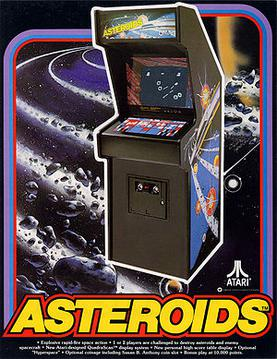
\includegraphics[height=1.3\textwidth]{images/Asteroids-arcadegame.jpg}\hfill
    \end{minipage}
    \hfill
    \begin{minipage}{0.66\textwidth}
        \hfill 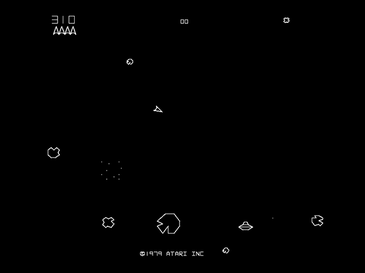
\includegraphics[height=0.65\textwidth]{images/atariasteroids-screenshot.png}
    \end{minipage}
    \caption{Atari Asteroids --- Promotional flyer cover~\cite{asteroidsflyer}
    and gameplay screenshot~\cite{asteroidsscreenshot}.}
\end{figure}

The game can be described as followed:
\say{A perfect synergy between simplicity and intense gameplay, the game has players using buttons to thrust a spaceship around an asteroid field. When one rock is shot, it breaks into smaller ones, often flying off in different directions at different speeds\ldots{} Every so often flying saucers enter the screen, intent on the player’s destruction.} \cite{aboutasteroids}
Its world comprises rocks (asteroids, in three sizes), projectiles,
flying saucers (large and small, trying to shoot the player) and the ship, controlled by the player,
trying to survive and gain score points by shooting down rocks and flying saucers.
There are a few features that we are omitting, like sound effects, some animations,
and several minor gameplay details. But we still need to handle input, simulate simple physics,
detect collisions, spawn entities, keep score, transition between the game
and its menus, and then render everything.



% ====================================
% CHAPTER 2 - About apecs
% ====================================
\chapter{Using the apecs library --- hAsteroids}
\label{chptr:hasteroids}

\section{About apecs}
\label{sect:apecs}
\say{Apecs: a fast, type-driven Entity\textendash{}Component\textendash{}System library for game programming} \cite{apecsrepo}
is one of the more recently released libraries.
Entity\textendash{}Component\textendash{}System (or ECS) is a data-oriented architectural pattern often
used in video game engines to represent the game world state.
In a true ECS, a game object or an \textbf{entity} is only an ID number,
and data is attached to it by being stored under that ID. This data is
organized into \textbf{components}, which are then stored in separate
lists with other components of the same type from other entities \cite{mediumecs}. This can
be represented as a table where every column is its own list or array
(see Table~\ref{tab:ecsexamp}). Then we define game logic as \textbf{systems}
--- a set of functions that operate on certain components regardless of the
entity as a whole. A typical example of a system is adding an entity's velocity
to its position for every entity with both of those components.
ECS usually provide better performance than object-oriented designs
because of their increased data locality --- a system needs to load into memory
only components that are relevant for it, not the whole \emph{objects}
as it would be with OOP \cite{apecspaper}.
\begin{table}[htp]
  \begin{tabularx}{320pt}{|r|lllX|}
    \toprule
    Entity & Position & Velocity & Type of Unit & Ammunition \\
    \midrule
    0 & $(4,2)$ & $(0,0)$ & Player   & 314\\
    1 & $(5,1)$ & $(1,1)$ & Enemy    & -- \\
    2 & $(2,2)$ & $(1,0)$ & Enemy    & -- \\
    3 & $(2,3)$ & --      & Obstacle & -- \\
    \bottomrule
  \end{tabularx}
  \caption{A simple example of ECS represented by a table.}
  \label{tab:ecsexamp}
\end{table}

And since both Unity and Unreal Engine use Entity\textendash{}Component design,
we chose apecs as the current state-of-the-art Haskell library
for the traction it has received in the community despite
it not being the only ECS library in existence.\footnote{
The making of the Ecstasy library was actually inspired by
author's issues with apecs as she explains on her blog \cite{whyecstasy}.
}

\begin{listing}[H]
\caption{Defining instance of \inlinehs{Component}.}
\begin{haskell}
newtype Position = Position (Double, Double)
instance Component Position where
    type Storage Position = Map Position
\end{haskell}
\label{lst:component}
\end{listing}

To write a game using apecs we must define \textbf{components} and \textbf{systems}.
Systems also create new \textbf{entities},
as creating them means to write some components under a new ID.

First, defining a \textbf{component} means to define an instance of the typeclass
\inlinehs{Component}, as we see in the Listing~\ref{lst:component}.
The \inlinehs{Component} class
requires us to state how we want to store the given component
by assigning a type alias to the specific storage type.
We can define our \inlinehs{Stores} or use one of those provided
with the library: \inlinehs{Map}, \inlinehs{Unique}, \inlinehs{Global} (and \inlinehs{Cashe}).
With \inlinehs{Map}, there can be multiple components of that type,
each belonging to a particular entity.
With \inlinehs{Unique}, at most one component may exist
belonging to a particular entity. Furthermore,
with \inlinehs{Global}, at most one component instance can exist,
and it belongs to the special \inlinehs{global} entity together
with every other entity at the same time. Finally, we call \inlinehs{makeWorld},
which uses Template Haskell to generate \inlinehs{World} product type
along with \inlinehs{initWorld} function and instances of the \inlinehs{Has}
typeclass needed for altering contents of \inlinehs{World} through
the other functions in apecs. The resulting \inlinehs{World}
may look close to something as shown in Listing~\ref{lst:world}.

\begin{listing}[H]
\caption{Simplified world state type example.}
\begin{haskell}
data World =
    World
    { record1 :: !(Unique Player)
    , record2 :: !(Map Enemy)
    , record3 :: !(Map Bullet)
    , record4 :: !(Map Position)
    , record5 :: !(Global Time)
    }
\end{haskell}
\label{lst:world}
\end{listing}

\textbf{System} in apecs is anything with the \inlinehs{SystemT w m a} return type, which
means that it may alter the world state.
One such \say{micro-system} is the \inlinehs{newEntity} function, which
accepts a tuple of components and adds them into their records under a new ID.
% \begin{haskell}
% newEntity ( Ship $ pi / 2 * 3
%           , Position $ V2 0 0
%           , Velocity $ V2 0 0
%           )
% \end{haskell}
More noteworthy functions to build systems are the component map functions
shown in the Listing~\ref{lst:cmaps}. They are the means of altering the world state.
\begin{listing}[H]
\caption{Component maps documentation \cite{apecsdocs}.}
\begin{haskell}
-- 'w' is the world type, 'm' is a monad,
-- 'cx','cy' and 'c' are tuples of components

-- | Maps a function over all entities
--   with a cx, and writes their cy.
cmap :: forall w m cx cy.
    (Get w m cx, Members w m cx, Set w m cy) =>
    (cx -> cy) -> SystemT w m ()
-- | Monadically iterates over all entities
--   with a cx, and writes their cy.
cmapM :: forall w m cx cy.
    (Get w m cx, Set w m cy, Members w m cx) =>
    (cx -> SystemT w m cy) -> SystemT w m ()
-- | Monadically iterates over all entities with a cx
cmapM_ :: forall w m c.
    (Get w m c, Members w m c) =>
    (c -> SystemT w m ()) -> SystemT w m ()
\end{haskell}
\label{lst:cmaps}
\end{listing}
\inlinehs{cmap} accepts a function that takes a tuple of components
and returns some other tuple of components. It internally iterates
over entities with at least those components matching the mapped
function's input tuple and writes the output tuple components
to those entities. \inlinehs{cmapM} works similarly
only as its name suggests the mapped function returns the component
tuple wrapped in the system monad, which allows it to execute side effects.
Furthermore, with \inlinehs{cmaM_} there is no direct writing, only side effects.



\section{Writing of hAsteroids}

In this section, we outline how we used apecs in the hAsteroids game.
For the exact implementation, please refer to the attached source files
in the hAsteroids directory.\footnote{
Attachment structure is briefly described in Appendix~\ref{app:attach}.}
Figure~\ref{fig:hasteroidsmodules} shows project's modules with loosely indicated
dependencies --- upper modules may have direct dependencies on the lower modules,
arrows show most important ones.
\begin{figure}[hbt!]
    \centering
    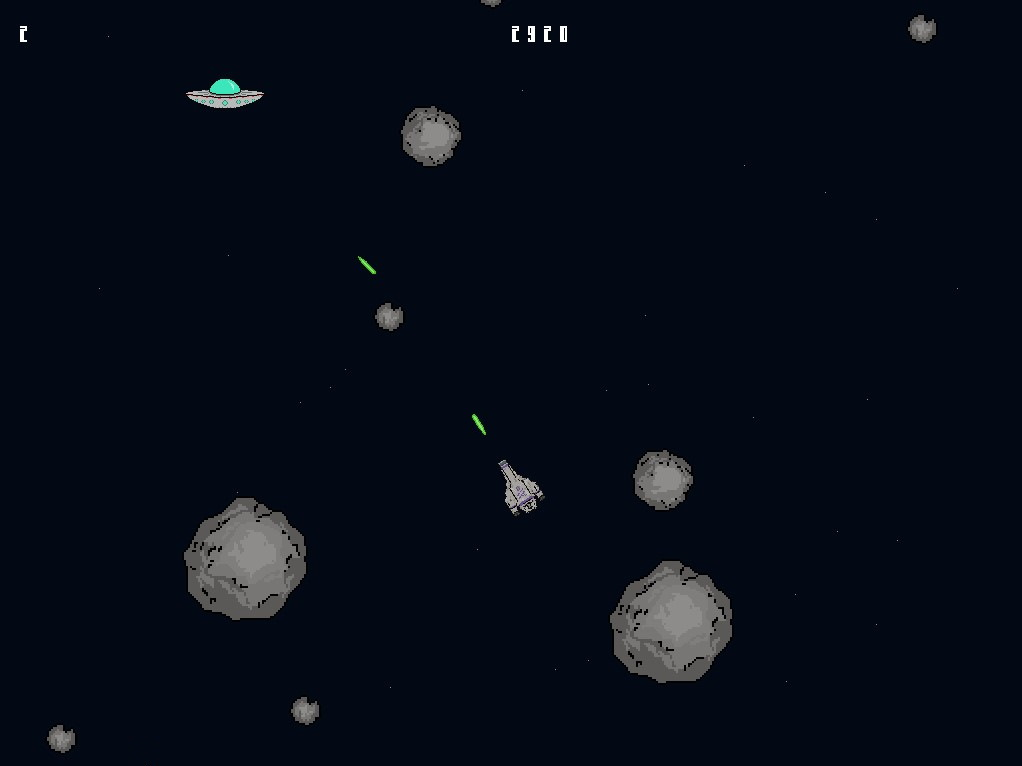
\includegraphics[width=0.7 \textwidth]{images/hasteroids-screenshot.jpg}
    \caption{A screenshot of hAsteroids gameplay.}
    \label{fig:hasteroidsscreenshot}
\end{figure}

\begin{figure}
    \centering
    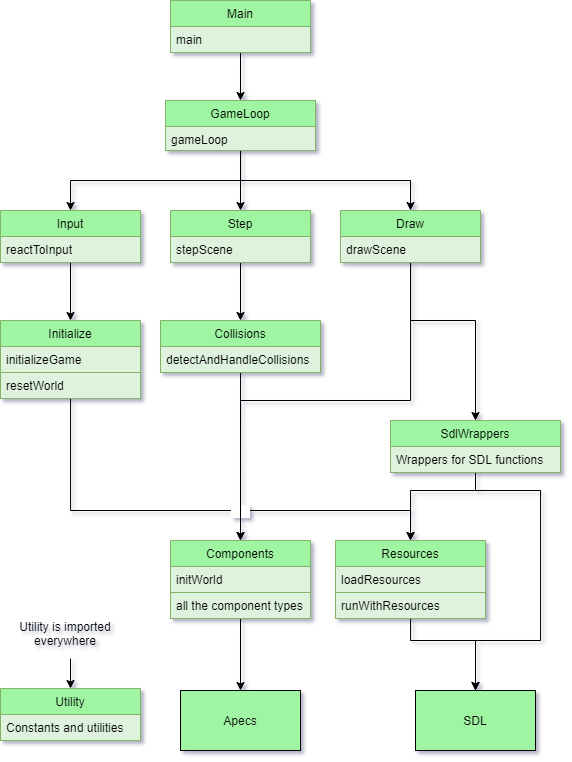
\includegraphics[width=\textwidth]{images/modules.png}
    \caption{hAsteroids module structure.}
    \label{fig:hasteroidsmodules}
\end{figure}


% components
\subsection{Components in hAsteroids}
There are more approaches to designing components but in hAsteroids,
we have three categories of components: \say{marker} components,
\say{shared} components, and \say{control} components. Marker components serve two purposes:
they contain information that is unique for a given type of game object,
and that way, they also mark an entity as that object.
Shared components include characteristics that are shared by more types
of game objects, like position. Lastly, control components are all global
and are used in one way or another to control the run of the game and the transitions between scenes.

hAsteroids has one \inlinehs{Unique} marker component called \inlinehs{Ship},
which marks an entity representing the player's ship and stores
the angle of the direction the ship is facing. The three other marker
components are \inlinehs{Map} stored. They are \inlinehs{Asteroid} — holding
asteroid size — \inlinehs{Ufo} — holding saucer size and a countdown
to the next UFO's shot being fired — and \inlinehs{Bullet} — storing whether
the player or a UFO shot it. Next, there are the shared components
\inlinehs{Position}, \inlinehs{Velocity} and \inlinehs{TimeToLive}
and several \inlinehs{Global} control ones like \inlinehs{ShipLives},
\inlinehs{ShipState}, \inlinehs{GameLoopState}, \inlinehs{WaveTime} and few others.
Table~\ref{tab:entities} shows which game object types should have which components;
however, it cannot be enforced by types due to the nature of ECS.

\begin{table}[hbt]
  \begin{tabularx}{\textwidth}{|r|X|}
    \toprule
    Object & Components \\
    \midrule
    % Ship     & \inlinehs{Position}, \inlinehs{Velocity}, \inlinehs{Ship} \\
    % UFO      & \inlinehs{Position}, \inlinehs{Velocity}, \inlinehs{TimeToLive}, \inlinehs{Ufo} \\
    % Bullet   & \inlinehs{Position}, \inlinehs{Velocity}, \inlinehs{TimeToLive}, \inlinehs{Bullet} \\
    % Asteroid & \inlinehs{Position}, \inlinehs{Velocity}, \inlinehs{Asteroid} \\
    Ship     & \texttt{Position}, \texttt{Velocity}, \texttt{Ship} \\
    UFO      & \texttt{Position}, \texttt{Velocity}, \texttt{TimeToLive}, \texttt{Ufo} \\
    Bullet   & \texttt{Position}, \texttt{Velocity}, \texttt{TimeToLive}, \texttt{Bullet} \\
    Asteroid & \texttt{Position}, \texttt{Velocity}, \texttt{Asteroid} \\
    \bottomrule
  \end{tabularx}
  \caption{Game objects and their components.}
  \label{tab:entities}
\end{table}


% the outer level
\subsection{Initialization and looping}
\label{sect:initialization}
The \inlinehs{main} function is the entry point of the program. It first initializes
the SDL libraries and then creates a window and a renderer. Next, using \inlinehs{loadResources},
it loads object textures into a hash map, prerenders fonts saving them into another
hash map, and wraps it all together with the renderer and a few stateful random generators
into one product type called \inlinehs{Resources}. Then the game world with our
components is created by calling \inlinehs{initWorld}, and together with resources,
it is passed to the \inlinehs{gameLoop} through a stack
of monad transformers (\inlinehs{SystemWithResources}). When the gameLoop quits,
the window is destroyed, and resources are freed.


% Systems
\subsection{Systems in hAsteroids}

\inlinehs{gameLoop} is one large compound system responsible for \textbf{updating} and \textbf{drawing}
the world and the menus every frame of the game. World updating is split
into two functions: \inlinehs{reactToInput} and \inlinehs{stepScene}.
The scene (a menu or the world) is then drawn by \inlinehs{drawScene}.
It also measures elapsed time every frame and calls \inlinehs{SDL.Delay} if it was
updated and drawn too quickly for the targeted 60 FPS.
This is then repeated until the player quits the game.

\subsubsection{\textbf{Reacting to input}}
\inlinehs{reactToInput} manages the state of the input, and as its name suggests,
reacts to it. Depending on the global \inlinehs{GameLoopState} component,
it either transitions between the states (\inlinehs{InMenu}, \inlinehs{Playing},
\inlinehs{Paused}, \inlinehs{GameOver}, \inlinehs{Quit}) or
when in the \inlinehs{Playing} state, it also allows the player to control the ship.
That is done by a \inlinehs{cmapM} that changes ship's angle,
increases its velocity, or creates a new bullet entity --- all conditioned by the input state.

\subsubsection{\textbf{Stepping the scene}}
\inlinehs{stepScene} takes care of simulating physics and game rules
over time when the loop is in the \inlinehs{Playing} state.
This is divided into a series of twelve function calls:

\begin{itemize}[\textendash]
    \item  \inlinehs{cmap $ stepKinetics dT}\\
    iterates over all entities and adds their velocity vector multiplied
    by time \inlinehs{dT} to their position vector and also takes care
    of wrapping the space --- if an entity flies out of the screen on one side,
    it comes back in from the other side.

    \item \inlinehs{cmap $ decelerateShip dT}\\
    simply applies deceleration to the ship by scaling down its velocity vector slightly.

    \item \inlinehs{cmapM $ stepShipState dT}\\
    is responsible for transitioning between ship states
    (\inlinehs{Alive}, \inlinehs{Exploding Int}, \inlinehs{Respawning Int},
    where the integers serve as countdown timers for the state transition)
    and the explosion animation.

    \item \inlinehs{cmapM_ $ ufosShoot dT}\\
    iterates over all \inlinehs{Ufo} components decrementing the time to
    shoot, and when it reaches 0, it creates a new \inlinehs{Bullet}.
    The algorithm for finding a shooting direction is different for the two UFO sizes.
    Small UFOs are more accurate than the large ones because the algorithm uses
    the law of sines to calculate the bullet trajectory based on the ship's current
    position and velocity. Large UFOs shoot in a quarter of $\pi$ increments
    towards the ship's current location.

    \item \inlinehs{awardLifeIf10000}\\
    increments ship's lives by 1 for reaching every 10\thinspace{}000 score points.

    \item \inlinehs{modify global $ \(WaveTime t) -> WaveTime $ t + dT}\\
    simply adds the frame delta time \inlinehs{dT} to the wave time counter.

    \item \inlinehs{spawnUfos}\\
    randomly creates new UFO entities on the left side of the screen,
    with the chances increasing as the time spent in one wave (\inlinehs{WaveTime}) passes.

    \item \inlinehs{spawnNewAsteroidWaveIfCleared}\\
    uses \inlinehs{cfold} from apecs to count all asteroids and
    when there are none it starts counting up using the \inlinehs{WavePauseTimer}.
    When the timer reaches 1500 it calls \inlinehs{spawnNewAsteroidWave}
    from the \inlinehs{Initialize} module, which uses the random stateful
    generators from the \inlinehs{WithResources} reader monad to create new asteroids.

    \item \inlinehs{cmap $ \(Ttl t) -> Ttl $ t - dT}\\
    simply subtracts the frame delta time \inlinehs{dT} from all the
    \inlinehs{TimeToLive} components.

    \item \inlinehs{destroyDeadBullets} and \inlinehs{destroyDeadUfos}\\
    use \inlinehs{cmapM_} to destroy all the components for entities that run out of \say{time to live}.

    \item \inlinehs{detectAndHandleCollisions}\\
    is defined in its own module \inlinehs{Collisions}.
    The collisions are detected and handled individually between each
    entity group. The general idea is that we use \inlinehs{cmapM_} inside of \inlinehs{cmapM_}
    as an equivalent of nested for loops. This way, for every asteroid,
    we iterate (or map) over all the other entities, checking for collision.
    We do the similar for the rest of the combination pairs,
    using in total $\binom{6}{2} = 6$ slighlty different collision detection algorithms.
    All the collisions are detected
    simply as a question of \say{is a point or any of the points inside of a rectangle,
    an ellipse or a circle.} A detected collision always results in some effect
    --- the colliding entities are removed, except an asteroid may break into two
    smaller ones if it is not already the smallest size, and
    in the case of the ship, one life is subtracted.
\end{itemize}

\subsubsection{\textbf{Drawing the scene}}
Once the scene is stepped, it is then \textbf{drawn} by the already mentioned \inlinehs{drawScene}
function from the \inlinehs{Draw} module. If the loop state is \inlinehs{InMenu} or
\inlinehs{GameOver}, only text is drawn on a cleared black screen. That is done by
\inlinehs{drawCenteredTexts}, which only calls a monadic \inlinehs{zipWith} with
\inlinehs{drawCenteredText} on a list of y coordinates and a list of text keys.
\inlinehs{drawCenteredText} itself then looks up the text texture in the
hash map that is part of the \inlinehs{WithResources} environment,
queries its width, and finally calls \inlinehs{drawText} with the coordinates
for the texture to be drawn centered.

When the loop is in the \inlinehs{Paused} state, there is text being drawn
as well as the world. Naturally, when the state is \inlinehs{Playing},
only the world is drawn. This is taken care of by \inlinehs{drawWorld},
which calls functions to draw the background, entities and the UI
(number of lives and the score). Entities are drawn using \inlinehs{cmapM_}
with a lambda function and a wrapper function around the \inlinehs{SDL.copy} and
\inlinehs{SDL.copyEx}, which renders the corresponding texture for every entity.


% Reflection
\section{Reflection}
\label{sect:apecsreflection}

From this example alone,
we learn that apecs makes game programming in Haskell surprisingly accessible.
Once we understand the ECS principle, every world modification is
\say{intuitively imperative} thanks to the \inlinehs{SystemT w m a} monad and
the component map functions. Any system side effects can be added
to an existing \inlinehs{cmap} call with a simple change of the return types
as demonstrated in Listing~\ref{lst:changingmind}.
\begin{listing}[H]
\begin{haskell}
-- steer and thrust
handleInput input =
    cmap $ \(Ship a, Velocity vel) ->
               ( Ship $ a + steering input
               , Velocity $ vel + thrust input a
               )
-- we realized that we also want to be able to pause the game
handleInput' input =
    cmapM $ \(Ship a, Velocity vel) -> do
                when (wasPressed input escapeKeycode)
                    (set global Paused)
                pure ( Ship $ a + steering input
                     , Velocity $ vel + thrust input a
                     )
\end{haskell}
\caption{We can easily switch between non-effectful and effectful calls.}
\label{lst:changingmind}
\end{listing}

Moreover, the \inlinehs{WithResources} reader monad provides easy
access to resources without passing them along everywhere as a function argument.

No less important is the fact that the game works.
The development experience was smooth, with no significant hiccups.
Because Haskell is a statically-typed high-level language, there is
no reason to worry about random invalid memory access making our game crash,
and everything is type-safe.

However, this approach is far from perfect. Handling collisions on an
individual basis would scale very poorly, so some universal interface would be better.
This could be achieved by defining a typeclass and its instances for the marker components.
More polymorphism could also differentiate functions that require the
\inlinehs{System} monad, the \inlinehs{WithResources} monad, or both.
In the current state, there are many functions, such as \inlinehs{reactToInput},
which do not use the resources but still have access to them since
everything returns the transformed \inlinehs{SystemWithResources} monad
that has \inlinehs{WithResources} inside of it. Furthermore,
said monad transformer stack\footnote{
\inlinehs{type SystemWithResources = SystemT World (ReaderT Resources IO)}
where \inlinehs{SystemT} is only a \inlinehs{newtype}
around \inlinehs{ReaderT} defined in apecs
}
includes \inlinehs{IO}, so any function with this type can perform
input or output effects, which goes against functional purity and nullifies
many of the reasons why one would choose Haskell as a language in the first place.

Another issue we observe is partially tied to the nature of ECS --- there
is no way to destroy all of an entity's components automatically in apecs.
One has to do destroy them explicitly. That way, nothing protects us
from accidentally adding a component to an entity that will never be destroyed.
This could be mitigated by creating helper functions for entity creation and destruction.

Overall, because apecs is so powerful, it makes it easy for the programmer to rely
on it too much and produce code that does not reach all the potential
benefits of purely functional programming.



% ====================================
% CHAPTER 3 - About functional style
% ====================================

\chapter{Focusing on functional purity --- pure-asteroids}
\label{chptr:purity}

\section{Game engines in purely functional style}
\label{sect:pureengines}

In the previous chapter, we see how a program in Haskell can still be
written in a very imperative style. 
This is certainly a valid approach and has its benefits, as we discuss
further in Chapter~\ref{chptr:evaluation}. However, for the second version of
Asteroids (project \emph{pure-asteroids}), we focus on functional purity,
clarity, and proper compartmentalization.

The design is inspired by a keynote \cite{carmackkeynote} of John Carmack, the co-founder
of id~Software and co-creator of the Doom and Quake games.%\cite{carmackbio}
At one point in the keynote, he talks about how he had been moving towards
a functional style of programming with \cpp{} and seeing the long-term benefits.
He also talked about his experiments with Haskell and his vision for multi-core
game logic. \say{State of where we're at right now with game code is that we run
all the game code in one thread because the idea of using locks to synchronize
amongst all of our current game code was just absolutely terrifying,} he says.
Then, explains how independent parallelism is much more feasible with pure
functions and how events can be used for interactions between the isolated groups.

The world-updating function can be split into individual sub-functions that update each group
of entities. Each sub-function is passed the game world and the group of entities, and
it returns the updated group; therefore, in Haskell, such function cannot affect
anything outside of the group it returns. For that reason, it could be easily run
in parallel, increasing the performance.

With this approach comes one more advantage
--- all entities are being updated based on the same image of the past state, meaning
it does not matter in what order entities are updated, the result will be the same.
This can be contrasted with a naive imperative approach, where entities are
updated sequentially in-place based on the current state. Such an approach may lead to
inconsistencies if, for example, two units attack each other at the exact same time.
Alternatively, to give an example from Asteroids, if a UFO and the ship shoot at each other
with an asteroid in between them, whichever bullet's collision is detected first
would destroy the bullet and the asteroid, and the other bullet would fly through,
killing either the UFO or the ship. However, the opposite approach comes with a caveat,
and that is the issue of two objects moving into a common space when they are not allowed to overlap.
John Carmack addresses this in his already mentioned keynote \cite{carmackkeynote} and
says it can be solved, for instance, by some kind of repulsion force. Fortunately, this
is a non-issue in Asteroids because all objects may overlap, usually causing a collision
and destruction.



% Writing of
\section{Writing of pure-asteroids}
\label{sect:pureimplementation}

\begin{figure}[hbt!]
    \centering
    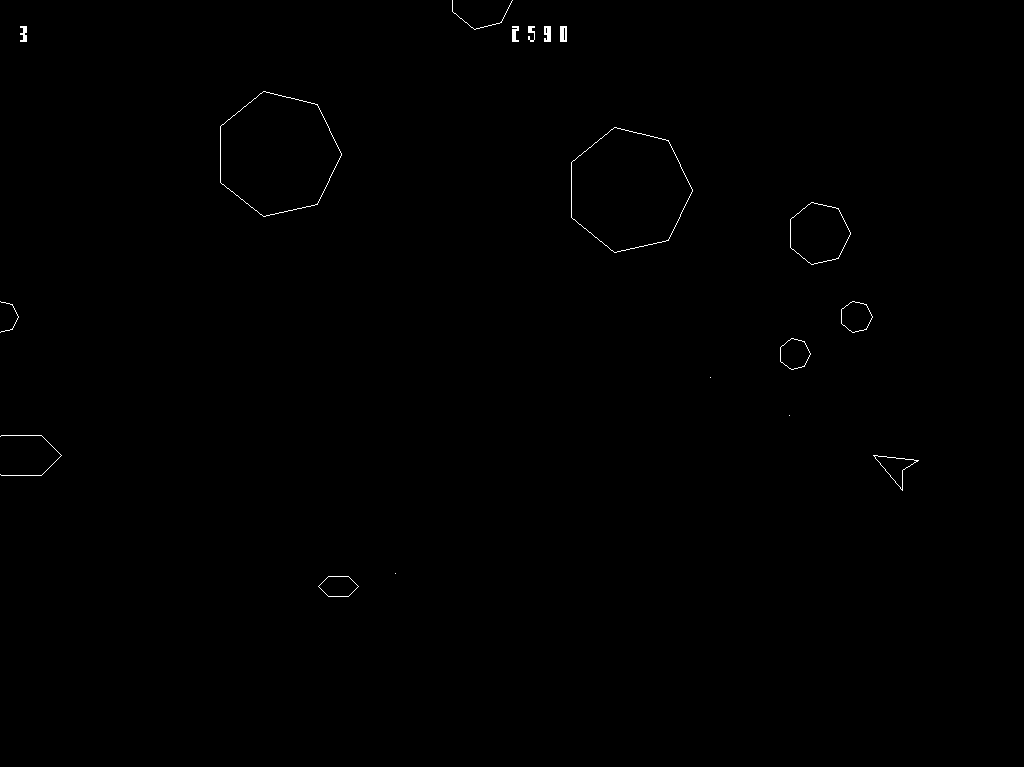
\includegraphics[width=0.6 \textwidth]{images/pure-screenshot.png}
    \caption{A screenshot of pure-asteroids gameplay.}
    \label{fig:pureasteroidsscreenshot}
\end{figure}

\noindent In this section, we describe how \emph{pure-asteroids} implements a pure style engine described
in the \hyperref[sect:pureengines]{previous section}.
For the exact implementation, please refer to the attached source files
in the pure-asteroids directory.\footnote{
Attachment structure is briefly described in Appendix~\ref{app:attach}.}
The program's main function is very similar to the one from
hAsteroids except for texture loading because pure-asteroids
draws vector graphics much like the original Asteroids. There is also no reader monad,
and \inlinehs{gameLoop} is passed everything explicitly as arguments.
The looping itself is also similar to hAsteroids, but naturally,
the world updating and drawing differ. The world state passes through
\inlinehs{processWorldEvents}, which fulfils all the requests from events,
through \inlinehs{stepWorld}, which simulates physics and game rules and generates new events,
\inlinehs{drawScene} draws it and \inlinehs{resetIfNewGame} returns a reinitialized
world only if the loop state is transitioning from \inlinehs{InMenu} to \inlinehs{Playing}.
This is illustrated in Figure~\ref{fig:worldeventsflow}.
Next, we describe the used \textbf{data structures} and then explain
how the \textbf{stepper function} and \textbf{event processing} use them.
\begin{figure}[h]
    \centering
    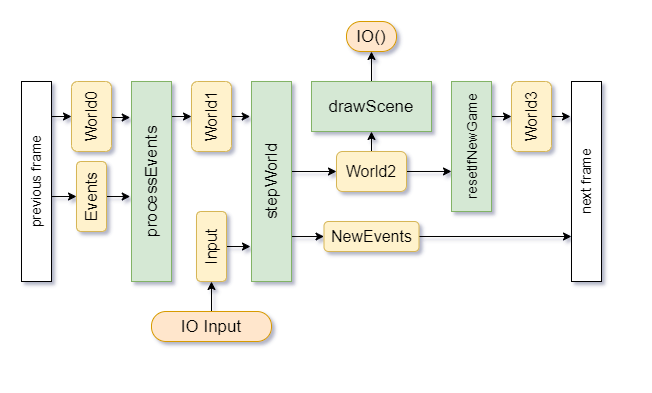
\includegraphics[width=\textwidth]{images/world-flow-detailed.png}
    \caption{Data flow of \inlinehs{gameLoop} in pure-asteroids.}
    \label{fig:worldeventsflow}
\end{figure}
% \begin{figure}
%     \centering
%     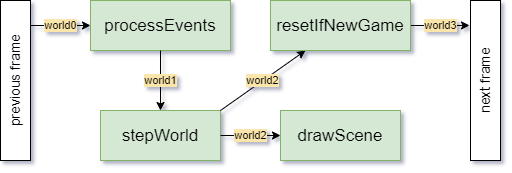
\includegraphics[width=\textwidth]{images/world-flow-basic.png}
%     \caption{The flow of world sate variable.}
%     \label{fig:worldflow}
% \end{figure}



\subsection{Data structures}

The two primary data structures, as already shown in Figure~\ref{fig:worldeventsflow},
are the world state represented by \inlinehs{World} and the events for communication
between entity groups represented by \inlinehs{WorldEvents}.

The definition of \inlinehs{World} can be seen in Listing~\ref{lst:pureworld}.
\inlinehs{World} contains separate groups of entities and some other state variables.
\inlinehs{Asteroids}, \inlinehs{Ufos} and \inlinehs{Bullets} are type
aliases for hash maps of the respective entities.
The entities themselves then contain similar data as components in hAsteroids,
only here, the data is all in one place, grouped by the game object.
Listing~\ref{lst:pureship} shows \inlinehs{Ship} definition as an example.
We can notice the preceding underscores in the record names. This is used
to generate lenses by using \inlinehs{makeLenses} from the \packagename{mtl} package
to facilitate easier data manipulation in our nested structures.

% Game World
\begin{listing}[H]
\begin{haskell}
-- | Game world state structure 
data World =
    World
    { _wShip      :: Ship 
    , _wAsteroids :: Asteroids
    , _wBullets   :: Bullets
    , _wUfos      :: Ufos
    , _wWaveTime  :: Time
    , _wWavePause :: Time
    , _wWaveNum   :: Int
    , _wScore     :: Score
    }
\end{haskell}
\caption{World structure in pure-asteroids.}
\label{lst:pureworld}
\end{listing}

% The Ship and its state
\begin{listing}[H]
\begin{haskell}
-- | Ship state structure
data Ship =
    Ship 
    { _sPosition :: Position
    , _sVelocity :: Velocity
    , _sAngle    :: Angle
    , _sLives    :: Int
    , _sState    :: ShipState
    }

data ShipState
    = ShipAlive
    | ShipExploding Time
    | ShipRespawning Time
\end{haskell}
\caption{The \inlinehs{Ship} representation in pure-asteroids.}
\label{lst:pureship}
\end{listing}
\pagebreak

Listing~\ref{lst:events} shows the event package type \inlinehs{WorldEvents}.
It also has an instance of \inlinehs{Monoid}, which allows us to collect the packages from
each entity group and combine them into one in the \textbf{stepper function}.
Then we distribute the events to their addressed entity groups in \textbf{event processing}.
The individual event types and the information they carry are described later,
with the functions that process them.

% World Events type
\begin{listing}[H]
\begin{haskell}
-- | Structure for event passing between entity groups
data WorldEvents =
    WorldEvents
    { _forAsteroids :: [AsteroidEvent]
    , _forShip      :: [ShipEvent]
    , _forUfos      :: [UfoEvent]
    , _forBullets   :: [BulletEvent]
    , _forScore     :: [ScoreEvent]
    }
\end{haskell}
\caption{The event package structure.}
\label{lst:events}
\end{listing}


% stepWorld
\subsection{Stepper function}
We can see the combining of event packages happen in the definition of \inlinehs{stepWorld}
in Listing~\ref{lst:purestepworld}. The events are returned by
the individual steppers of each entity group together with the stepped versions
of those groups. Note how lenses are used to \say{focus} on the contents of the world state
and change them with the setter operator \inlinehs{.~} or the function applicator \inlinehs{%~}
(or also the lens equivalent of \inlinehs{+=}).
Each \say{substepper} is compartmentalized and could be made to run in parallel.

% stepWorld definition
\begin{listing}[H]
\begin{haskell}
-- | Update the world
--   simulating physics and reacting to input
stepWorld :: Time -> InputState -> RandomStream Double -> World -> (WorldEvents, World)
stepWorld dT input rand oldW =
    let
        (eventsS, newShip)    = stepShip dT input oldW $ oldW ^. wShip
        (eventsB, newBullets) = stepBullets dT input oldW $ oldW ^. wBullets
        (eventsU, newUfos)    = stepUfos dT rand oldW $ oldW ^. wUfos
        (eventsScr, newScore) = stepScore dT $ oldW ^. wScore
    in
        (,) (eventsS <> eventsB <> eventsU <> eventsScr) $
        checkWave $
        oldW
          & wShip      .~ newShip
          & wAsteroids %~ stepAsteroids dT
          & wBullets   .~ newBullets
          & wUfos      .~ newUfos
          & wWaveTime  +~ dT
          & wScore     .~ newScore
\end{haskell}
\caption{The stepper function.}
\label{lst:purestepworld}
\end{listing}

Figure~\ref{fig:entitygroups} shows which events, represented by their value constructors,
entities may send to others.
The working of the individual substeppers can be summarized as follows:
\begin{itemize}[--]
    \item \inlinehs{stepShip}\\
    changes the ship's angle and velocity based on the input and updates its position.
    It also detects collisions with asteroids and UFOs. In the case of a collision,
    it adds an event with the entity's id to the event package. Moreover, it subtracts
    a life in that case and changes the ship's state attribute, which results in
    a spinning explosion animation next few frames. Then a position reset followed by
    a second of invincibility. All of that is done in \inlinehs{stepShip} conditioned by the state.

    \item \inlinehs{stepAsteroids}\\
    does not send any events, only updates the position of all asteroids.

    \item \inlinehs{stepBullets}\\
    first filters out bullets that run out of time to live (TTL), and then it uses \inlinehs{traverse}
    to call \inlinehs{stepBullet} on all the bullets, collecting all events as an
    \inlinehs{Applicative} side effect.\footnote{
    We use the predefined \inlinehs{instance Monoid a => Applicative ((,) a)},
    where \inlinehs{a} is our \inlinehs{WorldEvents} package.}
    \inlinehs{stepBullet} then updates position, decrements TTL, or marks the bullet for
    deletion by setting TTL to 0 if a collision was detected. Bullets check for collisions
    with everybody else and send them events, together with a reward event for \inlinehs{Score}
    if the bullet was shot by the ship.
    Finally, we insert a new bullet if the space bar was pressed.

    \item \inlinehs{stepUfos}\\
    operates similarly to \inlinehs{stepBullets}. It filters out the ones out of TTL,
    traverses over all of them, and at the end, it randomly inserts a new UFO.
    During the traversal, positions, TTLs, and \say{time-to-shoot} counters are updated.
    It checks for collisions with asteroids and sends an event together with setting its TTL
    to 0 if that happens. Additionally, when the time-to-shoot timer reaches 0, it is refreshed
    to 2000~ms, and an event is sent to \inlinehs{Bullets} as a request to insert their shot
    with information about the direction and position. The direction is calculated using
    one of the same two algorithms as in hAsteroids.

    \item \inlinehs{stepScore}\\
    sends an event to the ship, awarding it with an extra life for every 10\thinspace{}000 points gained.
\end{itemize}
After that, \inlinehs{checkWave} takes care of spawning new waves of asteroids,
and then the stepped world is paired with the collected, generated events and returned.

% Entity interactions figure
\begin{figure}
    \centering
    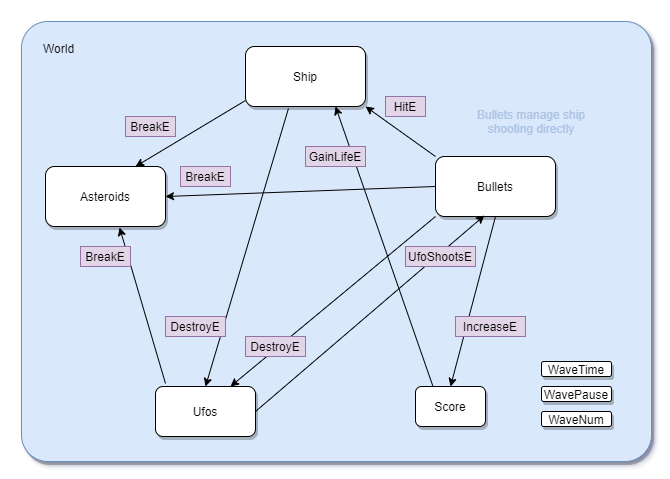
\includegraphics[width=0.9 \textwidth]{images/entity-relationships-transparent-bg.png}
    \caption{Entity groups and their interactions.}
    \label{fig:entitygroups}
\end{figure}



\subsection{Event processing function}

In Listing~\ref{lst:pureprocessevents}, we can see the implementation of
event processing and again the use of lenses.
Similar to \inlinehs{stepWorld}, the work is compartmentalized
and could be made to run in parallel, even though there are not that many
events sent each frame in the current game.
% processWorldEvents definition
\begin{listing}
\begin{haskell}
processWorldEvents :: WorldEvents -> World -> World
processWorldEvents events world =
    world
      & wAsteroids %~ processAsteroidsEvents
                        (events ^. forAsteroids)
      & wShip      %~ processShipEvents
                        (events ^. forShip)
      & wUfos      %~ processUfosEvents
                        (events ^. forUfos)
      & wBullets   %~ processBulletEvents
                        (events ^. forBullets)
      & wScore     %~ processScoreEvents
                        (events ^. forScore)
\end{haskell}
\caption{The event processing function.}
\label{lst:pureprocessevents}
\end{listing}
\inlinehs{processWorldEvents} calls the individual event processors and passes them
their share of events. All of those work in a similar fashion: they use \inlinehs{foldl}
or \inlinehs{foldr} to fold all the events into the changed entity collection.
Here is an example of \inlinehs{UfoEvent} processing:
\begin{haskell}
processUfosEvents :: [UfoEvent] -> Ufos -> Ufos
processUfosEvents =
    flip $ foldr resolveDestruction
    where
        resolveDestruction (DestroyE idU) =
            HM.delete idU
\end{haskell}

The rest of the \say{subprocessors} differ in the function used to apply an event to the collection
to fulfil the request. All the possible events are also shown in
Figure~\ref{fig:entitygroups}, here we list their value constructor definitions
and briefly describe what they cause or request:
\begin{itemize}[--]
    \item \inlinehs{BreakE Int}\\
    causes the addressed asteroid to break into two or to be deleted if it is the smallest size.
    
    \item \inlinehs{HitE | GainLifeE}\\
    causes the ship to either lose a life and set the state to \inlinehs{Exploding}
    or to gain an extra life.
    
    \item \inlinehs{DestroyE Int}\\
    targets a UFO and simply requests its deletion.
    
    \item \inlinehs{UfoShootsE Position Velocity}\\
    gives the \inlinehs{Bullets} all the needed information for inserting a new
    bullet shot by UFO.
    
    \item \inlinehs{IncreaseE Int}\\
    says how many points should be added to the current score.
\end{itemize}



% Reflection
\section{Reflection}
\label{sect:purereflection}

Overall, pure-asteroids achieves what it set out to do --- we can observe
many of the benefits described in Section~\ref{sect:whyfpmatters}.
Because it does not use much abstraction, the code is perceivably safer and more expressive.
For example, we can look at \inlinehs{shoot} from the \inlinehs{Step.Bullets} module:
\begin{haskell}
shoot :: InputState -> World -> Bullets -> Bullets
shoot input w =
    if wasPressed input spaceKeycode
        then insertBullet
        else id
\end{haskell}
We immediately see from the name and the type signature that the function presumably
somehow alters the collection of \inlinehs{Bullet}s based on the input and that
the alteration is probably adding a new bullet, which is confirmed by looking
at the following four lines of light code. Moreover, this also means that it is \emph{the only thing}
the function can do --- it clearly cannot change the state of the ship, read from a file,
or render a white square on the screen.

It also incorporates what we may call \emph{functional elegance}.
Throughout the code base, we use functions like \inlinehs{map}, \inlinehs{filter},
\inlinehs{fold}, \inlinehs{traverse} and many others that Haskell programmers are familiar
with and which make the code brief and save us time.

Most importantly, as we have demonstrated, the design could be adapted to
use parallelism, which we expect would increase performance.
Parallel computation would be especially beneficial if the game were of a larger scale
and the computation were more demanding --- for instance, collision detection
in pure-asteroids is elementary, but it could be improved by using more complicated algorithms.

However, even though we could use parallelism, the scalability of our design is somewhat lacking.
It would be appropriate to use more typeclasses in general --- a class interface for
collision detection, stepping, communication via events, and using resources.
Pure-asteroids is too explicit, which makes it relatively rigid
--- adding a random number generator to a bottom-level
function requires passing it from the top level
as an argument through the whole function chain. Besides, the long type signatures of the
top-level functions make them less clear.

Ultimately, we see that explicitness is good but has its boundaries
and that some level of abstraction is needed. 
It should also be pointed out that designing the complete engine from scratch
took a significant effort, despite the development being smooth and the final
product working well.




% ========================================
% CHAPTER 4 - Analysis of imperativeness
% ========================================

\chapter{Analyzing an existing \cpp{} implementation}
\label{chptr:impasteroids}

This chapter, describes the imperative implementation that we later
use to compare against in Chapter~\ref{chptr:evaluation}.
We shall refer to it as \say{imp-asteroids}.
It was made by Jason Halverson, and its GitHub repository can be found at
\url{https://github.com/Halverson-Jason/Asteroids}. We created a fork of
this repository with a branch named \inlinecpp{organized}~\cite{impasteroidsrepo}
with the original game with reorganized and reformatted files for convenience.

We acknowledge that \cpp{} may not be the most relevant comparison
as there are other choices for making a simple game quickly.
However, we chose this example because it does not use any third-party engines.
That way, we can easily compare it to our implementations
without an extra layer of complexity.

Furthermore, the options available all turned out to be of generally lower quality.
Like our two implementations, this version is not flawless,\footnote{
The game was made as a school assignment, and from the commented \inlinecpp{TODO}s
throughout the code, we can judge that there were certain time limitations.}
but we point out its mistakes and present them as a possible outcome of this language choice.
Though, the choice does not imply nor condition such an outcome.
\begin{figure}[H]
    \centering
    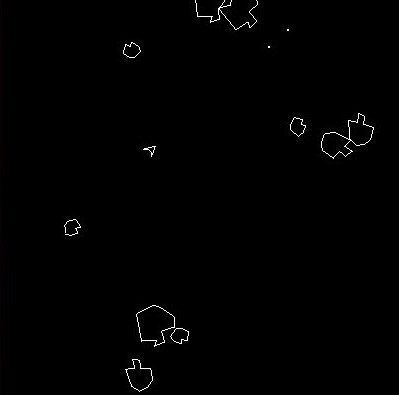
\includegraphics[width=0.5 \textwidth]{images/imperative-asteroids.jpg}
    \caption{A screenshot of imp-asteroids.}
    \label{fig:impscreenshot}
\end{figure}


\pagebreak
\section{Differences in features}

This version differs from our two implementations in many ways,
other than the language and style used. We want to list the most significant ones here:
\begin{itemize}[--]
    \item It uses GLUT with a custom wrapper instead of SDL to draw vector graphics.
    \item Asteroids have more jagged shapes, rotate as they fly around,
    and the ship has a thrust animation.
    \item There are no menus, lives or score and the ship does not respawn.
    \item Waves do not increase in the number of asteroids.
    \item It does not have UFOs.
    \item Physics are closer to the original.
    \item It does not support variable refresh rate.
    Every frame updates the world by a single implicit unit of time.
\end{itemize}


\section{How it works}
The \inlinecpp{main} function is very simple. It constructs a new \inlinecpp{Game} object,
and a new \inlinecpp{Interface} object. Then it calls \inlinecpp{run} on the \inlinecpp{Interface}
passing it a pointer the the game object and a call back function.
The callback function shown in Listing~\ref{lst:impcallback} is then registered in GLUT
as the \inlinecpp{drawCallback}. That way it gets called from within \inlinecpp{glutMainLoop}
every frame.

\begin{listing}
\begin{cppblock}
void callBack(const Interface *pUI, void *p)
{
    Game *pGame = (Game *)p;

    pGame->advance();
    pGame->handleInput(*pUI);
    pGame->draw(*pUI);
}
\end{cppblock}
\caption{The core of imp-asteroids main loop.}
\label{lst:impcallback}
\end{listing}

The \inlinecpp{Game} object has a pointer to a \inlinecpp{Ship} object, an \inlinecpp{std::vector}
of \inlinecpp{Bullet} pointers, and an \inlinecpp{std::list} of \inlinecpp{Asteroid} pointers.
All the entity objects inherit from the class \inlinecpp{FlyingObject}, which provides position, rotation,
velocity, position updating (\inlinecpp{FlyingObject::advance()}),
a universal collision detection using radii,
and a few more miscellaneous attributes and methods.

\subsubsection{Stepping the world}
\inlinecpp{Game::advance()} is used to \say{advance} the world by one unit of time.
It calls these subfunctions to do so:
\begin{itemize}[--]
    \item \inlinecpp{Game::advanceBullets()}\\
    iterates over all the bullet pointers and calls \inlinecpp{advance} on them.

    \item \inlinecpp{Game::advanceAsteroids()}\\
    iterates over all the asteroid pointers and calls \inlinecpp{advance} on them.
    If the collection is empty, it inserts five new large asteroids.

    \item \inlinecpp{Game::advanceShip()}\\
    calls \inlinecpp{advance} on the ship.

    \item \inlinecpp{Game::handleCollisions()}\\
    iterates over every bullet and asteroid, and in the case of a collision it
    marks the bullet and the asteroid as dead, and creates new asteroids
    unless the destroyed one was already the smallest size.

    \item \inlinecpp{Game::cleanUpZombies()}\\
    checks if entities are dead and deletes them if so.
    Delaying the deletion prevents inconsistencies caused by serial
    updating of entities --- this way the order of iteration does not matter.
\end{itemize}

\subsubsection{Input handling}
\inlinecpp{Game::handleInput} checks through the \inlinecpp{Interface} object
whether the controls were pressed, and calls ship's appropriate methods or
inserts a new bullet as necessary.

\subsubsection{Rendering}
Finally, \inlinecpp{Game::draw} iterates over all the entities and calls their
\inlinecpp{draw} methods.
Only unexpected thing is the call of \inlinecpp{Bullet::setHealth} for all the bullets.
This method decrements the bullet's health every frame and marks it as dead
if the value gets to zero, similarly to TTL in our implementations.



\section{Reflection}
The game benefits from OOP as most of the top-level function (method) calls
are very intuitive. It also avoids duplicity of code by using inheritance for position updating
and polymorphism for universal collision detection.
It offers decent scalability in adding new entities or features;
however, there should be separate manager classes for each entity group.
We also used \inlinecpp{valgrind} for memory profiling, and it discovered
several usages of uninitialized values and memory leaks.

We also dislike GLUT's use of callbacks and global state, making things
confusing and difficult to test. Although, we understand that
the goal of this particular implementation was not to be overly ambitious
about scalability since the game is straightforward.
Moreover, side effects can be present anywhere, and mutation of the game's state
also is not limited very strongly. This is naturally a challenge for all imperative languages.

One could argue that this is not an issue and that programmers only need be
more competent about their usage of these powers. To combat this, the already quoted
John Carmack talked about how being a technical director over millions of lines of code,
he saw how \say{everything that is syntactically legal that the compiler will accept,
will eventually wind up in your codebase.} \cite{carmackkeynote} He also said that
\say{it's just amazing how many mistakes, and how bad programmers can be.}~\cite{carmackkeynote}
Because programmers are, after all, only humans, systems like the functional paradigm,
that limit their ability to be \say{bad} can be of great use, as we demonstrate
further in the following chapter.



% ====================================
% CHAPTER 5 - Final COMPARISON
% ====================================

\chapter{Evaluation of the approaches}
\label{chptr:evaluation}

In this chapter, we first compare Haskell to imperative languages in general or specifically to \cpp{},
often referencing back to the promised benefits of Haskell from Section~\ref{sect:whyfpmatters}.
Then we discuss the conflicts observed in the comparisons and their possible solutions.


\section{Comparison}

This section compares the three example implementations or, more broadly, Haskell and
imperative languages represented by \cpp{}.
For this, we reference the previous chapters about individual implementations.
It is important to note that \cpp{} is by no means meant
to represent imperative languages fully; even less so is the chosen imperative implementation
of Asteroids (further referred to as \textit{imp-asteroids}) meant to represent
the ideal game design in \cpp{}. Not only it has flaws, but it is also an even
simpler version of the original game in some ways than our two implementations.
We try to address this in especially relevant places;
in others, it is left out for the sake of conciseness and readability.

The comparison is organized by qualities important in game development:
flexibility and scalability, expressiveness and safeness, development costs, performance.
The section is then closed off by an additional comparison of state abstraction
and few statistical observations about the codebases.



\subsection{Flexibility and scalability}

Both \textbf{hAsteroids} and \textbf{imp-asteroids} are very flexible designs.
Because in hAsteroids, the monad return type of most functions is not very
restrictive at all, we can add in and take away effects or resources with ease.
Similarly, the imperative version is highly flexible in this sense. When it comes
to scalability, both do decently well. Adding new game objects in hAsteroids can be done by
defining more components and needed systems. Already existing components and systems can be reused
like \inlinehs{Position}, \inlinehs{Velocity} and \inlinehs{stepKinetics}.
One issue would be the expansion of collision detection,
which is done on an individual basis; therefore, the amount of work
would grow linearly with an increasing number of game objects.
Imp-asteroids does better in this regard --- kinetic properties can
be inherited from \inlinecpp{FlyingObject} as well as the ability to detect collisions.
The issue here might be if we wanted to inherit only parts of \inlinecpp{FlyingObject}.
Also, with a large scale, the safeness becomes more of a concern for both games
--- more on that in the following subsection.

We have already described how \textbf{pure-asteroids} are rather rigid because of
their lack of abstraction. Scalability is also worse than the other two since
adding new objects would require writing their whole \say{substepper} and
new event paths, and collision detection is handled similarly to hAsteroids.



\subsection{Expressiveness and safeness}

As we have already discussed in Chapter~\ref{chap:motivationandmethods},
functional languages are designed to be clearer (\emph{expressiveness})
and to better control side effects (\emph{safeness}) than conventional
imperative languages. Now the imperative code can be even more or less unsafe
depending on its type system. \cpp{} is mostly strongly and statically typed,
providing a certain amount of assurance. Some other languages are not.
This can protect us from trying to add an object to a number, for instance.

Many languages also take various steps towards controlling side effects.
One such example could be the \inlinecpp{const} keyword used to define a variable
that cannot be mutated. In \cpp{}, this keyword can also be used on methods
to prevent them from changing the state of the object, allowing us to call these
methods even on \inlinecpp{const} objects. Usage of this keyword would prevent
the author of imp-asteroids from writing the drawing function seen in Listing~\ref{lst:baddraw} that
unexpectedly also changes the state of bullets.
However, languages like Java or Python do not support immutable objects,
and we can see how control of side effects, in general, is a \say{plan B} in the imperative paradigm.
\begin{listing}[H]
\begin{cppblock}
void Game::draw(const Interface &ui) {

    /* ... other objects are drawn... */
    
    for (int i = 0; i < bullets.size(); i++) {
        if (bullets[i]->isAlive()) {
            bullets[i]->draw();
            bullets[i]->setHealth(); // a setter?!
        }
    }
}
\end{cppblock}
\caption{The danger of side effects.}
\label{lst:baddraw}
\end{listing}

Conversely, since Haskell originated as an academic language,
functional purity was allowed to be plan A, and having
side effects was actually plan B in this case.
We saw how this, together with the type system, works out well for expressiveness and clarity
in the example of \textbf{pure-asteroids}, as showcased on an exemplary function
at the beginning of Section~\ref{sect:purereflection}.
And because all variables are immutable, change is made explicit as a \emph{new} returned value
that we pass forward.
Moreover, any input/output side effects are clearly separated by the \inlinehs{IO} monad,
and the rest of the code is entirely deterministic, which alltogether with strong static typing
makes for a very safe language --- not only there is less potential sources of bugs, but the
correctness of a program is \emph{easier to perceive} and argue about.

That is if used well --- \textbf{hAsteroids} turned out to be a very interesting game.
apecs makes game programming in Haskell approachable and provides
excellent performance by being \emph{strict and imperative}. This inner imperativeness
makes purity sort of a plan B again, and the programmer has to be clever about using monad polymorphism
if they want to keep \say{the danger of \inlinehs{IO}} contained. This has occurred to us in the middle
of the hAsteroids development process, so we decided to embrace it and see where it leads.
If we had redesigned the types, we could have reached better safeness and even expressiveness.
However, with the game world state abstracted, it is still not always clear what functions do
when applied through \inlinehs{cmapM} or \inlinehs{cmapM_}.



\subsection{Development costs}

The purpose of any language feature can ultimately be seen as reducing the cost of development.\footnote{
% By development costs, we mean mainly development speed and comfort.
By development costs, we mean mainly time and endured frustration. Generally speaking,
any piece of software can be written in any language; what differs is the cost.
}
The already discussed Haskell features all bring the costs down in certain scenarios, but there is more
that we want to look at through the lens of development speed and comfort.
Both \textbf{pure-asteroids} and \textbf{hAsteroids} more or less benefit from these.

\subsubsection{Interpreter}
One of such features is \textbf{GHCi}, \say{GHC's interactive environment,
in which Haskell expressions can be interactively evaluated,
and programs can be interpreted.} \cite{ghciwiki}
Haskell is a compiled language that comes with an interpreter as well.
An interpreter allows us to test short expressions quickly, either to try something new or to
run bits of already existing code. \texttt{GHCi} can also print the types of expressions
or information about typeclasses. We have used the interpreter frequently during development
for reminding ourselves of type signatures, testing vector manipulation, and more.


\subsubsection{Functional elegance}
Furthermore, there is many predefined high-order functions like
\inlinehs{map}, \inlinehs{filter}, \inlinehs{foldl} and so forth. This way, a part of the
job is already done, and we only need to provide the elemental function to fold with, for instance.
This, together with being able to apply functions partially, allows us to write
very \textbf{brief and elegant code}. In Listing~\ref{lst:elegance},
we can see asteroid stepper implementations
from imp-asteroids and pure-asteroids.\footnote{
The \cpp{} version also spawns a new wave of asteroids if the current has been cleared.
That part of the code was omitted as it is irrelevant for the example.
} The Haskell version uses \inlinehs{map} with a partially applied function,
while too being only partially applied. Granted, other languages have structures
to make this sort of task at least slightly more elegant too
and even \cpp{} itself has \inlinecpp{std::for_each},
which could be used to make this piece of code more concise. However, this characteristic extends
to the whole Haskell code base --- in both of our games there is only three instances
of explicit recursion in total: the game loops and \inlinehs{drawLines} in pure-asteroids.
This is rather impressive considering the games have to manipulate collections of events,
textures, entities, components and others. More examples of elegant code are appended at the end
of this thesis in Appendix~\ref{app:elegance}.
We also address conciseness further, in Subsection~\ref{sect:codestats} (Code statistics).
\begin{listing}[H]
\begin{minted}[fontsize=\small, breaklines]{cpp}
// C++
void Game::advanceAsteroids() {
    for (list<Asteroid*>::iterator it = asteroids.begin();
         it != asteroids.end(); it++) {
            (*it)->advance();
    }
}
\end{minted}

\begin{minted}[fontsize=\small, breaklines]{haskell}
-- Haskell
stepAsteroids :: Time -> Asteroids -> Asteroids
stepAsteroids dT = HM.map (stepAsteroid dT)
\end{minted}
\caption{Asteroid stepping with for-loop and map.}
\label{lst:elegance}
\end{listing}


\subsubsection{Testing and debugging}
Another benefit discussed at the beginning in Section~\ref{sect:whyfpmatters}
is the \textbf{ease of testing and debugging}. Testing a pure function is as simple or as complicated
as the function's parameters and its output. Testing an impure function is
theoretically nearly impossible to do \emph{exhaustively} since without looking at
its definition, we do not know whether it reads from a file or not, for instance.
Practically, we do not need to be completely exhaustive and can make assumptions;
however, those unchecked assumptions are the weak spots that may cause problems.

Due to time constraints, Haskell's safeness and the simple nature of Asteroids,
we did not use any automated tests during our development. Still, to substantiate
the claim of easier testing we look at the two functions\footnotemark in Listing~\ref{lst:testingexamp},
and consider how we would go about testing them. 
\footnotetext{ The examples are again taken from imp-asteroids and pure-asteroids.
\inlinehs{stepBullets} has been simplified in this case. The real version also
inserts new bullets based on the input state, which happens elsewhere in the \cpp{} implementation.
}
\begin{listing}
\begin{minted}[fontsize=\small, breaklines]{cpp}
// C++
void Game::advanceBullets() {
    for (int i = 0; i < bullets.size(); i++) {
        if (bullets[i]->isAlive()) {
            bullets[i]->advance();
            if (!isOnScreen(bullets[i]->getPoint())) {
                bullets[i]->kill();
            }
        }
    }
}
\end{minted}

\begin{minted}[fontsize=\small, breaklines]{haskell}
-- Haskell
stepBullets :: Time -> World -> Bullets -> (WorldEvents, Bullets)
stepBullets dT w =
    traverse (stepBullet dT w) . filterDeadBullets
\end{minted}

\caption{Impure and pure stepping of bullets.}
\label{lst:testingexamp}
\end{listing}
To test \inlinehs{stepBullets} we need to provide three arguments. First is a simple
integer, and the other two are much more complex but still could be generated randomly using
Haskell QuickCheck or provided \say{manually}. The only effect produced is the returned
pair that can be checked for correctness by other functions. On the contrary, to test
\inlinecpp{advanceBullets} we need to set up a \inlinecpp{Game} object with its contents,
many of which are \inlinecpp{private}. That requires refactoring, and
the same applies to testing the state after \inlinecpp{advanceBullets} has been called.
Additionally, we may want to test not only whether the collection of bullets has
changed correctly but also whether the rest of the state is correct.

\textbf{hAsteroids} is no better as the test needs to run inside of the \inlinehs{SystemT w m a} monad,
where we set up components using \inlinehs{newEntity} function and then after running
tested system checking the validity of all the components.

\subsubsection{Tools}
Lastly, an obvious disadvantage is the fact that writing a game in Haskell
is still largely a pioneering process. There is a decent amount of existing general tools,
one of them being the already described interpreter,
which can also be used to set up breakpoints and step through evaluation.
More extensive debuggers like Hat exist as well. We used Stack for easy management of
the package and its dependencies. However, even some general tools such as a robust IDE
are easier to find for other languages, and in terms of game development specific tools,
there are not many besides the several libraries like apecs listed in Section~\ref{sect:existing}.
This can be contrasted with the complete, general engines that come included with 
tools for the whole development pipeline, such as Unity.

This was expected, and it turned out not to be an issue as our example game was
very simple. Although, we can imagine that with a larger game, we would start
to feel the need for more tools.



\subsection{Performance}

Performance in games is very important since there is a real minimum requirement
given by desired frame rate and the player's expected hardware. A game can offer
a decent experience at 60 FPS, which gives us roughly 16 ms to do any computation
we need for a single frame. With smaller games, this is plenty, but as the entity
counts grow and rules get more complex, performance optimization becomes essential.
For that reason, we want to compare the performance of our implementations and
the tools available to optimize it.

We put together simple \textbf{benchmarking} versions of all three games and ran them
to find how many frames can be rendered in a given time in similar situations.\footnote{
The benchmarking versions can be found in their respective GitHub repositories
on a branch called \texttt{bench}:\\
\url{https://github.com/honzaflash/cpp-asteroids/tree/bench}\\
\url{https://github.com/honzaflash/ba-thesis/tree/bench/hAsteroids}\\
\url{https://github.com/honzaflash/ba-thesis/tree/bench/pure-asteroids}
}
The games were altered to spawn various, abnormal quantities of asteroids and
run for ten seconds with the ship constantly spinning and shooting one bullet per frame.
Note that the results are rather illustrational as the differences between games were not controlled
very well: imp-asteroids uses GLUT with the FPS limited to a maximum of 59, because of issues
with \inlinecpp{stack exec} seemingly not running the programs at all on Windows,
the Haskell games were run in the interpreter, hAsteroids renders
textures instead of drawing vectors like the other two, and there are other minor differences.
The benchmark was run at least three times for every asteroid count, and the median is shown
in the results in Table~\ref{tab:benchfps}.

\begin{table}[H]
  \begin{tabularx}{\textwidth}{|r|llX|}
    \toprule
    Asteroid count & \textbf{imp-asteroids} & \textbf{hAsteroids}\footnotemark & \textbf{pure-asteroids}\footnotemark[\value{footnote}] \\
    \midrule
    10\thinspace{}000 & 41 & 2   & 1   \\
    500   & 59 & 30  & 16    \\
    250   & 59 & 46  & 23    \\
    100   & 59 & 55  & 37 \\
    50    & 59 & 74  & 92 \\
    25    & 59 & 117 & 140 \\
    10    & 59 & 141 & 154 \\
    % 5 + 200 UFOs & -- & 8 & 83 \\ % fascinating but no time for diagnosing/analysis :'(
    \bottomrule
  \end{tabularx}
  \caption{Average FPS in the benchmarks.}
  \label{tab:benchfps}
\end{table}
\footnotetext{hAsteroids and pure-asteroids were run in the interpreter
due to a problem with \inlinecpp{stack exec} on Windows.}

We ran the benchmark for 100 asteroids also in a virtual machine with Ubuntu,
where \inlinehs{stack exec} worked normally, and the results were quite different
even if we account for the slower \say{virtual hardware}:
46, 21, and 34 FPS respectively for imp-asteroids, hAsteroids, and pure-asteroids.
From these results, with all three games being compiled, we can assume,
what is said to be true for Haskell in other fields,
that its performance is mostly comparable to \cpp{}.
Unfortunately, we did not have time to diagnose why apecs performed so poorly in this case.
However, when comparing the two versions (hAsteroids and pure-asteroids)
running in GHCi on a physical machine,
hAsteroids with apecs does outperform pure-asteroids by up to 100~\% for high entity counts.
This was expected as apecs provides a data-oriented design that optimizes data locality in memory.

Worthy of note is also the profiling we did on the runs in Ubuntu.
Interestingly, we found out that drawing in hAsteroids accounts for less
used time and allocated memory than in pure-asteroids.\footnotemark{} This eliminates the
possibility of hAsteroids being bottlenecked by drawing textures instead of vectors.
Most importantly, it showed that neither of the games had issues with Garbage Collection (GC)
as this can become a problem with larger lazy systems.
The productivity reported by the \mintinline{console}{-s} profiling flag was 99.1~\%
for hAsteroids and 97.6~\% for pure-asteroids,
meaning GC is not causing any meaningful delays in our games.
\footnotetext{The profiling results can be found on the mentioned
\texttt{bench} branch of our GitHub repository:
\url{https://github.com/honzaflash/ba-thesis/tree/bench/pure-asteroids/results} and
\url{https://github.com/honzaflash/ba-thesis/tree/bench/hAsteroids/results}.
Specifically, the profiling of cost centers is in folders \texttt{opt-p}.}

This brings us to the \textbf{tools} available and ease of \textbf{optimization} in general.
As mentioned in the previous subsection, there are various tools, including
profilers for Haskell, but \cpp{} will have a larger variety. Another advantage
for \cpp{} in this discipline is its low-level access to hardware and memory management.
Generally, the less abstracted code is easier to optimize since it is closer to
what the CPU will actually execute. With more abstraction, more work must be
done to find out what the CPU does in the end. This is especially the case for Haskell,
which has a high level of abstraction and during compilation goes through \emph{three} intermediate
languages, therefore if one desires to see how the code gets \say{unabstracted}, he must
first learn at least the first of the intermediate languages (Core).
To make up for this at least partially, as we have also stated before,
GHC can do a lot of optimizing on its own, and purely functional code is also easier
to execute in parallel and concurrently, which Haskell is very good at.



\subsection{State abstraction}
\label{sect:stateabstraction}
One of the largest differences between the implementations is how they model the game's state.
Through this prism, we can see once again how \textbf{hAsteroids} and \textbf{imp-asteroids}
are very similar. As we have mentioned before, because of the abstraction,
the code in hAsteroids has a certain amount of imperative style, and that includes the state
of the game world kept in a monad. Similarly, despite \cpp{} having a lower-level
approach to memory and some other things, the object-oriented paradigm allows us
to abstract the state in a relatively elegant way. Object's attributes
define its current state, which is implicitly passed to any of its methods.
% \begin{cppblock}
% // this:
% strt o2(); // construct instance of strt struct
% set(o2, true); // call a function
% // can be abstracted into this:
% obj o1(); // construct instance of obj class
% o1.set(true); // call a method
% \end{cppblock}

The monad state is technically pure because, in reality,
its change is only a computation hidden behind the \inlinehs{>>=} operator
that passes the change as a \emph{new} value forward without any mutation,
and the operator itself then can be further hidden using the \inlinehs{do} block.\footnote{
Reminder: \inlinehs{do str <- getLine; putStr str} is a shorthand for
\inlinehs{getLine >>= (\str -> putStr str)}
}
But from a practical standpoint, there is only a little difference between a monad state
and an object's state. Just as an object gives a context to a method's side effects,
a state monad gives context to the monadic computation's side effects.
In the same way that an object stored in a single variable is changed, a monad state
can change without any outer signs. Listing~\ref{lst:state} shows how similar in appearance
are the main game loops of hAsteroids and imp-asteroids.

\begin{listing}[H]
\begin{haskell}
-- gameLoop returns SystemWithResources ()
reactToInput deltaTime
stepScene deltaTime
drawScene
\end{haskell}
\begin{cppblock}
// pGame is a pointer to Game object
pGame->advance();
pGame->handleInput(*pUI);
pGame->draw(*pUI);
\end{cppblock}
\caption{Cores of the main loops in hAsteroids and imp-asteroids.}
\label{lst:state}
\end{listing}

This brings us to the argument of why we want to avoid mutability in the first place.
Mutability makes code harder to reason about, easier to make mistakes in, and
very difficult to run in parallel. Granted, since the state monad is technically
pure, the hidden syntax will not allow shared mutability,
which is what makes parallel systems complicated.
With that in mind, it also makes some things much simpler to program.

As we have already pointed out, \textbf{pure-asteroids} steers clear of monads when possible,
modeling the state explicitly. This does indeed make things easier to reason about,
but it was much more complicated to write.
We discuss this need for balance later, in Section~\ref{sect:dilemmas} about the observed dilemmas.



\subsection{Code statistics}
\label{sect:codestats}

As a bonus, we include few simple statistics about code length.
We counted the lines, words\footnote{
\mintinline{console}{wc} defines a word
as a sequence of any printable characters delimited by white space.
}
and characters using the \mintinline{console}{wc} command.
Then we plotted the total line counts (Figure~\ref{fig:codelength}) and
ratios between words, lines, and characters in each file (Figure~\ref{fig:codedensity})
using Python and \packagename{seaborn}. We must take into account the differences between
the implementations because imp-asteroids uses a custom drawing library
built around GLUT, which includes several lengthy line-drawing functions and
it is much more heavily commented,\footnote{
Using \mintinline{console}{grep} we found 850 lines of comments in the imp-asteroids project
and only 110 and 50 in hAsteroids and pure-asteroids.
}
but it also does not implement UFOs, score, ship lives, or menus.

\begin{figure}[H]
    \centering
    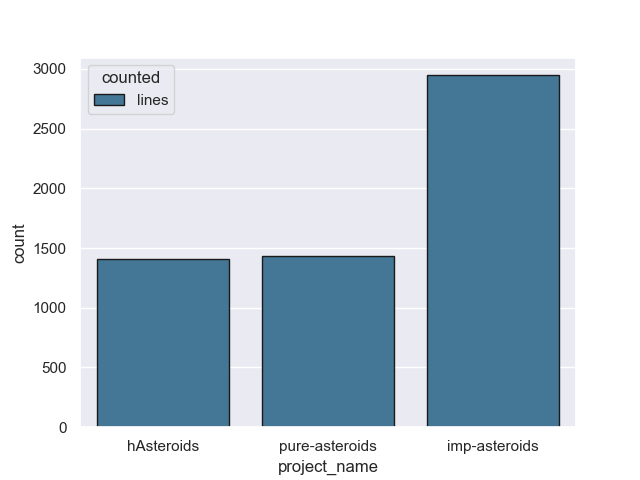
\includegraphics[width=0.9 \textwidth]{images/total_lines_by_project.png}
    % 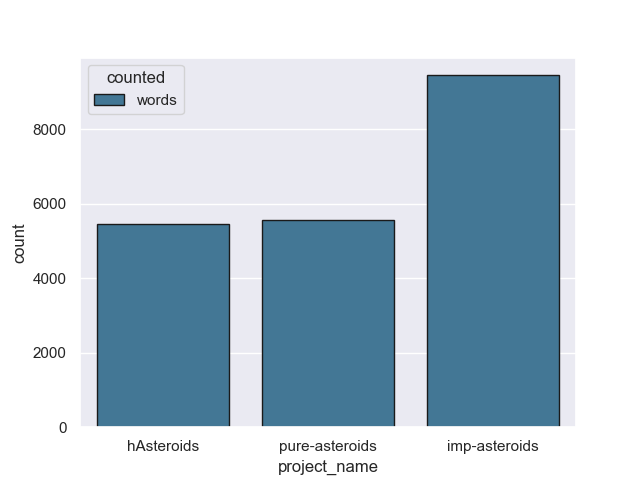
\includegraphics[width=0.49 \textwidth]{images/total_words_by_project.png}
    % 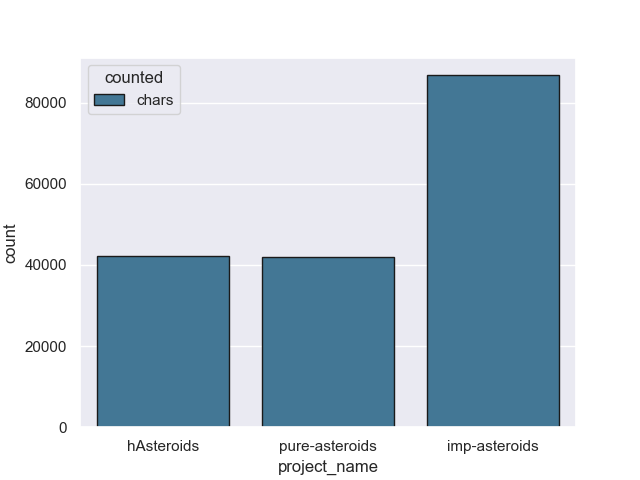
\includegraphics[width=0.49 \textwidth]{images/total_chars_by_project.png}
    \caption{Total number of lines by project.}
    \label{fig:codelength}
\end{figure}

\begin{figure}[H]
    \centering
    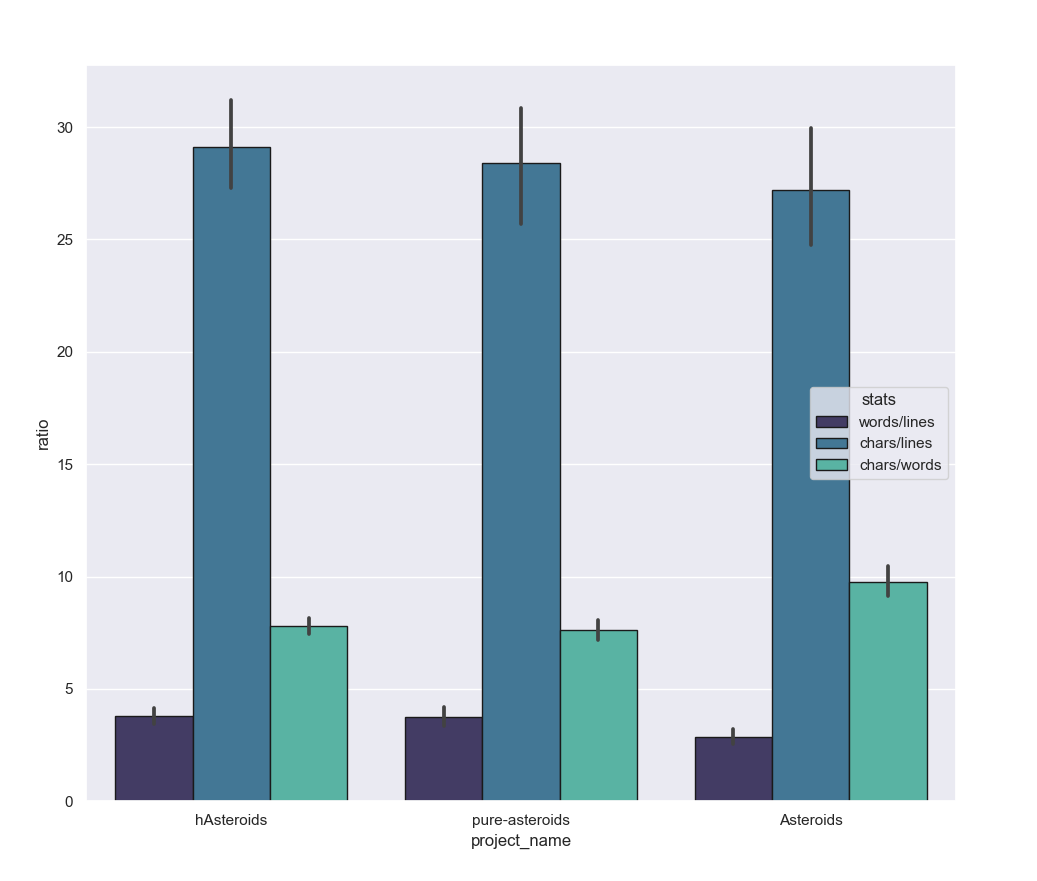
\includegraphics[width=\textwidth]{images/lwc_density_by_project.png}
    \caption{Code density by project.}
    \label{fig:codedensity}
\end{figure}

From the ratios in Figure~\ref{fig:codedensity}, we see that the codebases have a similar density;
therefore, we know it is not shorter lines inflating the total line count, but generally longer code.
This further supports the claim for Haskell's ability to be brief and concise.
We can also notice the slight, opposite tendencies of words per line and characters per word.
It would appear that in the \cpp{} code, words are longer, and there are fewer of them per line,
which can be explained by \mintinline{console}{wc} understanding strings like
\inlinecpp{asteroids.erase(it);} as one word as are also understood operators, more frequent in Haskell.

% ----------------------------------------------------------
% \subsection{pure-asteroids \vs hAsteroids}

% Both implementations are technically functional and both technically separate
% pure code from impure code with \inlinehs{IO}. But we have already mentioned
% how hAsteroids does not leverage the type system to do so.

% \subsection{hAsteroids \vs imp-asteroids}

% They are surprisingly similar.

% The difference (or lack there of??) between monad state and an implicit object state.
% Separation of effectful and uneffectful code - monad and const keyword.

% Haskell can be a very imperative language
% ------------------------------------------------------------




% Further discussion about programming theory
\section{Observed dilemmas}
\label{sect:dilemmas}

Here we discuss further the conflicts observed in the previous section
and suggest possible better compromises or solutions.
Namely we identify the tension between freedom of effects and safeness,
and between abstraction and explicitness.



\subsection{Freedom \vs safeness}
We saw examples of two extremes --- pure-asteroids with high safeness but low flexibility
and hAsteroids together with imp-asteroids with high flexibility but low safeness.
It may seem as though the two are mutually exclusive. However, we see another
characteristic hiding behind the flexibility label: \emph{freedom of side effects}
or unbound flexibility. That is what cannot be achieved
simultaneously as complete safeness rooted in control and limits.
Nevertheless, it definitely is possible to design a system that includes
constraints and control implemented in a relatively \emph{flexible} way.

We would argue that complete freedom is rarely even desirable.
It may be tolerable for smaller programs, possibly beneficial for simple scripts,
but for any more extensive application, programmers are taught \say{good practices} such as
\say{do not use global variables} and \say{do not use goto.}
A safe design can be achieved with good practices in a language like C,
but modern languages help us save time and money.
For this reason, it is of great use when a language supports robust control
of side effects.

Being able to compromise on unlimited side effects then, we believe that a reasonably flexible
system can by designed in Haskell, which is also very safe.
The addition of typeclasses was a great break through for Haskell and it is exactly this
feature that is used for good, modular, flexible and safe design of complex systems.
typeclasses are used to put constraints on types and can be also compounded,
that way the addition or removal of limits is relatively easy.
This not only helps controlling the return type, but can also help
with polymorphous arguments, making code more useful while staying safe.

We have criticized both of our own implementations for the way they model state
and pass along resources or access to \inlinehs{IO}. In Listing~\ref{lst:dreamdesign},
we can see a much better modular design suggestion, with types of the functions
using it in Listing~\ref{lst:usedream}. The complete working toy example
can be found in Appendix~\ref{app:classes}.
The main reader monad \inlinehs{WithResources} that allows functions
to access any of its contents and perform I/O
is restricted through polymorphism when subfunctions are called.
Constraints can be added to a function's type to grant access to more of the state or
or removed to limit it. Moreover, the \inlinehs{Resources} type and the typeclasses
could be expanded to accommodate for more resources.

\begin{listing}
\begin{haskell}
class MonadReader r m => TexturesReader r m where
    askForTextures :: m Textures

class MonadReader r m => RandomReader r m where
    askForRandom :: m RandGen

type WithResources a = ReaderT Resources IO a

data Resources =
    Res
    { textures :: Textures
    , random   :: RandGen
    }

instance Monad m => TexturesReader Resources (ReaderT Resources m) where
    askForTextures = asks textures

instance Monad m => RandomReader Resources (ReaderT Resources m) where
    askForRandom = asks random
\end{haskell}
\caption{Modular reader monad design.}
\label{lst:dreamdesign}
\end{listing}

\begin{listing}
\begin{haskell}
gameLoop :: World -> WithResources ()

step :: (RandomReader r m) => World -> m World

draw :: (MonadIO m, TexturesReader r m) => World -> m ()
\end{haskell}
\caption{Modular reader monad usage example.}
\label{lst:usedream}
\end{listing}

That way we can achieve decent system flexibility and still clearly compartmentalize
functions, limiting their access to what would be otherwise very close to a global,
imperative-like state. Included in that is the \say{evil} I/O access which can be added or removed
using the \inlinehs{MonadIO} class, which \inlinehs{ReaderT r IO} already has an instance for.




\subsection{Abstraction \vs explicitness}

In the previous subsection, we have already mentioned abstraction as the means
of gaining flexibility. Excessive abstraction results in too much flexibility,
as seen in hAsteroids. Conversely, too much explicitness leads to a lack of flexibility,
as seen in pure-asteroids.

However, despite explicitness being one of the key features that make functional
programming safer and easier to argue about, \emph{expressiveness} is the feature
more worthy of pursuing. We can see explicit data flow as the way of reaching
formal safeness, but it is expressiveness that helps us humans \emph{see it}.
Furthermore, explicitness does not imply expressiveness. The flow of data can be
described very precisely, but it may be so complicated that it does not make the code any clearer.
That is when abstraction steps in place, and when used wisely, it leads to a
more understandable code with fewer distractions. All of that, while in the background
still being technically pure and formally safe.

Figure~\ref{fig:4sides} illustrates the relationships between our four identified
foreground attributes and the two main background attributes we should be seeking.
\begin{figure}
    \centering
    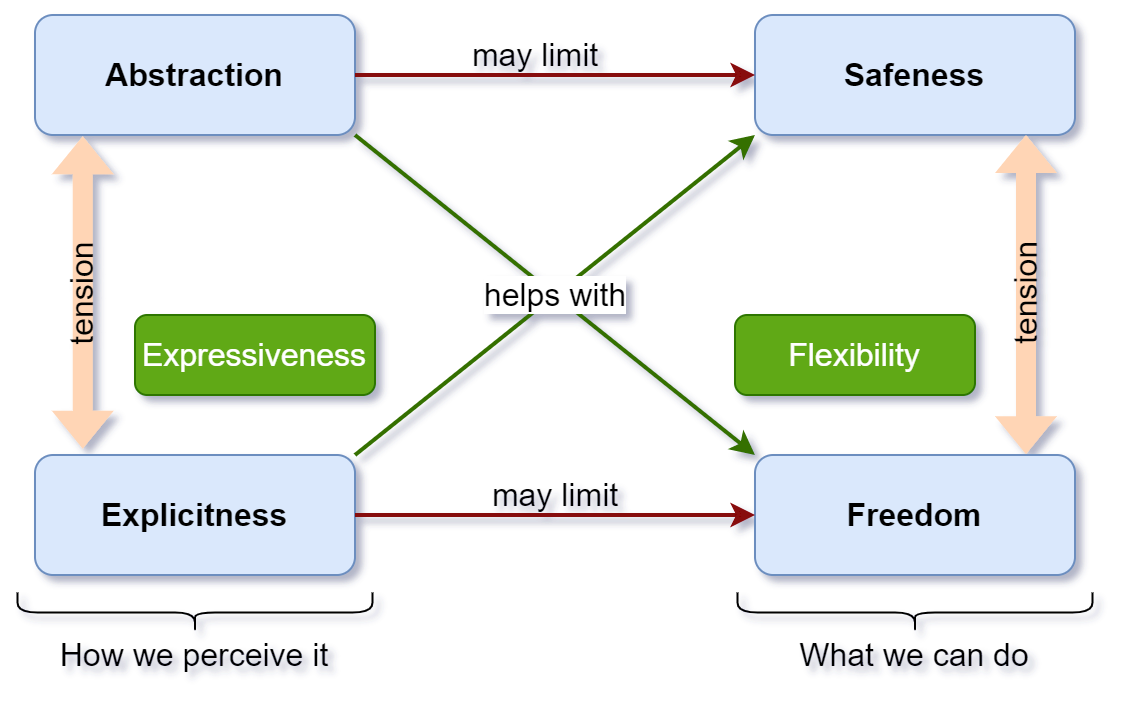
\includegraphics[width=\textwidth]{images/4sides-of-code.png}
    \caption{The four discussed qualities of design.}
    \label{fig:4sides}
\end{figure}

As with many things in life, we need to find a balance
between abstraction and explicitness so that our programs are still
easily provable to be correct while not being painful to write and modify.

When comparing the modeling of state in our three games in Subsection~\ref{sect:stateabstraction},
we have already pointed at how monads can emulate certain features of imperative languages,
and at the same time, stay technically pure.\footnotemark{} We see the example in listing
\ref{lst:usedream} as a good balance between abstraction and explicitness.
We lean towards modeling the game world state as an explicit variable since it is
the most important data structure. Mistakes in manipulation with it may be critical,
and as the likely most extensive data structure,
it could be highly beneficial to process it in parallel.

\footnotetext{Philip Wadler speaks more on
\say{combining the indulgences of impurity with the blessings of purity}
by using monads in his paper \textit{Comprehending Monads} \cite{wadlermonads}.}
% https://ncatlab.org/nlab/files/WadlerMonads.pdf

On the other hand, things like the state of a random number generator or other resources
meant only for reading, such as textures,\footnote{
In a larger game, textures may need to load dynamically; still, they are read-mostly data.
}
can be hidden in an appropriately named monad without an issue.
That way, we keep expressiveness but allow for flexibility.
As an additional supporting example, we consider the following two function types:
\begin{haskell}
step :: (RandomReader r m) => World -> m World

step' :: (RandomReader s m, WorldState s m) => m ()
\end{haskell}
One function takes a value of type \inlinehs{World} and returns
a new value of the same type under the influence of a reader monad.
While the other is obscurer and returns nothing but monadic effects.
At last, we admit that this is to an extent a matter of personal taste
and that some may prefer the effectful approach, despite what we have argued.\footnote{
An example of such an approach can be seen in the Dino Rush game,
described in the blog post \emph{A Game in Haskell - Dino Rush} \cite{dinorush} mentioned
previously in Section~\ref{sect:existing}.
}



% RECAP and final EVALUATION => moved to Conclusion
% \section{Summary}
% -- draft/notes

% it remains to be true even for game development that the code can be more expressive,
% safer and briefer --- there is a balance between abstraction and explicitness

% we have discussed the relationships of design qualities \ref{fig:4sides}

% classes can (and should) be used for polymorphism, increasing flexibility scalability and
% reducing code duplicity

% the language it self being very high-level and abstract can make it much more
% difficult to optimize, which is important for games --- languages like \cpp{} have the advantage

% it is said that Garbage Collection (GC) can be a problem in Haskell
% with interactive real-time applications, like video games, but it has been proven that
% it is ok for small to medium sized games
% --- paradox: pure functional design is great for long term and large scale,
% with Haskell the upfront cost is higher but the system produced is more likely to be of high quality

% We have rediscovered that Haskell can be very imperative, as explained by Simon P.~Jones and
% Philip Wadler in their paper \textit{Imperative Functional Programming}. \cite{imperativefp}
% % https://www.microsoft.com/en-us/research/wp-content/uploads/1993/01/imperative.pdf
% % https://youtu.be/re96UgMk6GQ?t=2089
% In that paper, they described for the first time, how monads could be used for input/output operations
% in lazy languages, and confirmed what we see in hAsteroids ---  with the \inlinehs{IO} monad
% Haskell can very closely resemble C. Yet, it keeps the benefits of functional style intact by
% clearly separating the imperative from the functional.

% perhaps also quote Carmack again, when he said how over the years of supervising
% hundreds of programmers working of thousands and thousands of lines of code, he saw that
% anything that is legal for the compiler will end up in your code base eventually
% --- Haskell's "brutal" functional purity is a win

% However, having limited tools and libraries at the upfront cost is high.
% Almost anyone in this area is a pioneer and
% the concept remains to be proven in practice on large scale games...




\chapter*{Conclusion}
\addcontentsline{toc}{chapter}{Conclusion}

In this thesis, we used two approaches to reimplement Asteroids by Atari in Haskell
resulting in two projects: hAsteroids and pure-asteroids.
We have described each implementation in Chapters~\ref{chptr:hasteroids} and~\ref{chptr:purity}.
Additionally, we picked an existing imperative reimplementation from GitHub and also
outlined its operation in Chapter~\ref{chptr:impasteroids}.
Then, in Chapter~\ref{chptr:evaluation}, we have compared the implementations
to determine whether the functional programming paradigm's
general benefits apply to game development.

We have gathered that our two approaches are opposite extremes on the spectrum
of abstraction and explicitness. Moreover, we discussed the relationship of those
characteristics with freedom of effects and safeness, concluding
that the focus should be on \emph{expressiveness} and \emph{flexibility}.
We argued that the latter two qualities are achieved by balancing the former two pairs
and showed how Haskell's typeclasses could be used together with monads
to achieve the desired balance.

We have rediscovered that Haskell can be very imperative, as explained by Simon P.~Jones
and Philip Wadler in their paper \textit{Imperative Functional Programming} \cite{imperativefp}.
In that paper, they described for the first time how monads could be used for input/output
operations in lazy languages and confirmed what we see as the result in hAsteroids --- with the
\inlinehs{IO} monad, Haskell can very closely resemble C. Yet, it keeps the
benefits of functional style intact by clearly separating the imperative from the functional.

Simultaneously, while the creators of Haskell argue for laziness, it can cause performance issues.
This happens when extensive unevaluated data accumulates and results in long delays caused
by the Garbage Collection (GC). This is especially of concern for video games where the time to
compute and render a frame is limited. Moreover, finding the sources of those \say{lazy memory leaks}
and doing other optimizations can be more challenging due to the language's strong abstraction.
However, we did not experience any problems with GC in our small-scale experiments.

Furthermore, we have found that the apecs library makes game programming in Haskell surprisingly
accessible. hAsteroids outperformed pure-asteroids by up to 100~\% for high entity counts
because of the Entity\textendash{}Component\textendash{}System design (a data-oriented design)
provided by apecs.
Creating pure-asteroids was more demanding, but its design is clearer, and it keeps
parallelism in mind. Even though it does not actually implement it, we paid attention
to making the architecture easy to modify for parallel computation.

Ultimately, we believe that the game's code can be more modular, in parts briefer,
easier to understand and to argue about its correctness than its imperative equivalent.
It does come at a higher upfront cost, especially considering the limited libraries and tools
(at least compared to the rest of the industry).
Regardless, we judge our development experience as very positive, and we would encourage others
interested in game programming to try Haskell themselves.
It may not currently be the safest way to bring a game to the market,
but at the bare minimum, it is a valuable learning experience and, at best,a step for the whole industry
towards better game engines with all of the perks of purely functional programming.

The benefits of purely functional design become most significant in the long term and large scale.
However, our examples are small in scale, and so it remains to be proven
in practice that our findings are applicable to more complex games
without running into issues with laziness, for instance.
Moreover, we would be curious to see whether adding the parallelism into pure-asteroids
would better the performance even at that scale, and further,
how it would compare to the data-oriented design of apecs as the entity counts grow.





% ====================================
%             Bibliography
% ====================================
\printbibliography[heading=bibintoc] %% Print the bibliography.



% \makeatletter\thesis@blocks@clear\makeatother
% \phantomsection %% Print the index and insert it into the
% \addcontentsline{toc}{chapter}{\indexname}
% \printindex



% ====================================
%             APPENDIX
% ====================================
\appendix %% Start the appendices.



\chapter{Electronic attachments}
\label{app:attach}

The implementations described in this thesis are attached with it
in an archive file. The contents of the archive are outlined here:
\medskip
\dirtree{%
.1 implementations.
.2 hAsteroids\DTcomment{the hAsteroids project root}.
.3 app.
.4 Main.hs\DTcomment{the entry point}.
.3 resources\DTcomment{textures and fonts}.
.3 src\DTcomment{library modules}.
.3 package.yaml\DTcomment{package details including dependencies}.
.3 stack.yaml\DTcomment{stack configuration}.
.2 pure-asteroids\DTcomment{the pure-asteroids project root}.
.3 app.
.4 Main.hs\DTcomment{the entry point}.
.3 resources\DTcomment{fonts}.
.3 src\DTcomment{library modules}.
.3 package.yaml\DTcomment{package details including dependencies}.
.3 stack.yaml\DTcomment{stack configuration}.
.2 README.md\DTcomment{readme file from the GitHub repository}.
}
\medskip
\noindent The build instructions are provided in the following appendix.\\
Latest version of projects can be found at \url{https://github.com/honzaflash/ba-thesis}.


\chapter{Build instructions}
The build process for both hAsteroids and pure-asteroids is very similar.
The following requirements must be met first.
\newcommand{\requirementitem}[1]{\noindent\textbf{#1}}

\medskip
\requirementitem{Haskell Tool Stack}
\begin{itemize}[\indent]
    \item Both games are projects managed using the Haskell Tool Stack;\footnote{
    About \mintinline{console}{stack}: \url{https://docs.haskellstack.org/en/stable/README/}
    } therefore, \mintinline{console}{stack} needs to be installed.
    We recommend running \mintinline{console}{stack upgrade} before attempting the build.
\end{itemize}

\requirementitem{SDL libraries}
\begin{itemize}[\indent]
    \item The used Haskell SDL bindings require the C libraries to be installed.
    Specifically, both projects need SDL and SDL\_ttf, and hAsteroids also uses SDL\_image 
    \item To install all three on Ubuntu, you can use this command:
    \begin{term}
    sudo apt install libsdl2-dev libsdl2-ttf-dev libsdl2-image-dev
    \end{term}
    
    \item To install all three on Windows with the help of \mintinline{console}{stack}:
    \begin{term}
    stack exec -- pacman -S mingw64/mingw-w64-x86_64-pkg-config mingw64/mingw-w64-x86_64-SDL2 mingw64/mingw-w64-x86_64-SDL2_ttf mingw64/mingw-w64-x86_64-SDL2_image
    \end{term}
\end{itemize}

\requirementitem{Operating System}
\begin{itemize}[\indent]
    \item Stack and SDL support Linux, Windows, and Mac~OS.
    The build was tested on Ubuntu~20.04 and Windows~10 build~19042.
\end{itemize}

\noindent With that, we can run \mintinline{console}{stack build} in the project's root directory.
This may take a while as \mintinline{console}{stack} downloads and installs all the dependencies.
To launch the game when project is built successfully,
execute \mintinline{console}{stack run} or \mintinline{console}{stack exec <name-of-the-executable>},
again, in the project's root directory.
We were unable to make \mintinline{console}{stack exec} work on Windows, so alternatively,
we can run \mintinline{console}{stack ghci} and then run the \inlinehs{main} function in GHCi.



\chapter{Additional code examples}

\section{Example of modular monad design using typeclasses}
\label{app:classes}

Here we list a working toy example, implementing the modular design
we outlined at the end of Section~\ref{sect:dilemmas}.

\begin{minted}[breaklines, linenos]{haskell}
{-# LANGUAGE FlexibleInstances #-}
{-# LANGUAGE MultiParamTypeClasses #-}

import Control.Monad.IO.Class
import Control.Monad.Reader

class MonadReader r m => TexturesReader r m where
    askForTextures :: m Textures

class MonadReader r m => RandomReader r m where
    askForRandom :: m RandGen

type WithResources a = ReaderT Resources IO a

type Textures = String
type RandGen = [Int]
data Resources =
    Res
    { textures :: Textures
    , random   :: RandGen
    }

instance Monad m => TexturesReader Resources (ReaderT Resources m) where
    askForTextures = asks textures

instance Monad m => RandomReader Resources (ReaderT Resources m) where
    askForRandom = asks random

newtype World = World Int deriving Show

main :: IO ()
main = do
    let world = World 10
    let resources = Res  
            { textures = "Current world state: "
            , random = [4, 2]
            }
    runReaderT (gameLoop world) resources  

gameLoop :: World -> WithResources ()
gameLopo w = do
    newW <- step w
    draw w
    quit <- liftIO $ getLine
    unless (quit == "q") $
        gameLoop newW

step :: (RandomReader r m) => World -> m World
step (World state)= do
    rand <- head <$> askForRandom
    -- performing I/O is illegal because 'm'
    -- does not have the MonadIO constraint on it
    -- liftIO $ putStrLn "C is the superior language"
    return $ World $ state + rand

draw :: (MonadIO m, TexturesReader r m) => World -> m ()
draw w = do
    t <- askForTextures
    liftIO $ putStrLn $ t ++ show w

\end{minted}


\pagebreak
\section{More examples of functional elegance}
\label{app:elegance}
Here we list a few more examples of elegant, concise code from our implementations.

\bigskip
\noindent No need for explicit iteration when loading textures:
\hrule
\begin{haskell}
loadTextures :: SDL.Renderer -> IO Textures
loadTextures r = ioOrDie "Failed to load textures" $
    HM.fromList <$> mapM mapPathToTexture keyPathList
    where
        mapPathToTexture = mapM (IMG.loadTexture r)
\end{haskell}

\bigskip
\noindent More map usage with partially evaluated functions:
\hrule
\begin{haskell}
-- | Calculates the ship vertices' positions
shipPoints :: Ship -> [V2 Double]
shipPoints s =
    map (+ sPos)
        [ -17 *^ (facing - perp facing) -- left
        ,  25 *^  facing                -- front tip
        , -17 *^ (facing + perp facing) -- right
        , -8  *^  facing                -- back point
        ]
    where
        sPos = s ^. sPosition . pVect
        facing = angle $ s ^. sAngle
\end{haskell}

\bigskip
\noindent Drawing an arbitrary number of textures with text stacked vertically,
utilizing laziness and list comprehension:
\hrule
\begin{haskell}
drawCenteredTexts :: SDL.Renderer -> Texts -> [TextKey] -> IO ()
drawCenteredTexts renderer texts =
    zipWithM_
        (drawCenteredText renderer texts)
        [100 * i | i <- [2..]]
\end{haskell}


\end{document}
